\documentclass[12pt, a4paper, oneside]{ctexbook}
\usepackage{amsmath, amsthm, amssymb, graphicx, float, hyperref, physics, esint}

\title{{\Huge{\textbf{狭义相对论专题}}}}
\author{李佳齐}
\date{\today}
\linespread{1.5}

\newtheorem{theorem}{定理}[section]
\newtheorem{definition}[theorem]{定义}
\newtheorem{lemma}[theorem]{引理}
\newtheorem{corollary}[theorem]{推论}
\newtheorem{example}[theorem]{例}
\newtheorem{proposition}[theorem]{命题}

\begin{document}
	
\maketitle

\pagenumbering{roman}
\setcounter{page}{1}

\begin{center}
	\Huge\textbf{序一}
\end{center}~\

这世界上有两大趣事:一是做学问,二是审美。就前者而言,虽说探索真理是人类永恒的追求,但具体到做学问,它本身会局限于社会和时代——与之不同,审美则是更一般更广泛的。往社会化的方面去说,人类社会的艺术门类是无国界的;而往本性、自然这方面去讲,“惟江上之清风与山间之明月,耳得之则为声,目遇之而成色,取之不尽用之不竭,是造物主之无尽臧也,而吾与子之所共适”。我以为人类喜欢蓝色的天空是进化的结果,那为何面对深邃的宇宙也能有如此的憧憬?所以,美,一定是一个超脱生命的更一般的存在。\par 
倘若一个人懂得审美的必要性,那他一定能从自然和社会领悟到许多;倘若一个人能够把审美的标准贯彻到工作,那他的成果一定值得欣赏;倘若这个人的工作刚好就是做学问,那这种学问一定堪称绝唱!物理就应该是这样的,尤其是相对论。\par 
我的水平顶多能讲出来狭义相对论的美感,这种美感,千人千面,尽在不言中,但我还是需要举个例子:假如我们学过高中物理,知道牛顿三定律,那么我们一定会感慨:牛顿力学竟然能解释日常生活的几乎全部力学问题,而且从技术上说单纯靠一个 $\vb*{F}=m\vb*{a}$ 就差不多了!这就是一种美感,你可能会说这属于还原论的思想,然后进行一番辩论,但不可否认的是,这真的很美!\par 
对于相对论,假如我们高中毕业了,高考物理考得还不错,大学可能不是物理专业的但是也学了普通物理,又接触了相对论,把公式都记下来了,甚至自己都推导了一遍——但你可能还是体会不到美感,毕竟面对下面这个洛伦兹变换的公式,谁能说这很美呢,第一反应肯定是头大吧!
\begin{equation}\label{e1}
	\left\{
	\begin{aligned}
		x'&=\gamma(x-vt)\\
		y'&=y\\
		z'&=z\\
		t'&=\gamma\qty(t-\dfrac{vx}{c^{2}})
	\end{aligned}
	\right.
\end{equation}
但其实,类似牛顿力学有 $\vb*{F}=m\vb*{a}$,狭义相对论也有一个非常简洁的数学公式,那就是洛伦兹变换:
\begin{equation}
	A'^{\mu}=\Lambda^{\mu}_{\nu}A^{\nu}
\end{equation}
第一,这个式子很简洁,就是一个线性变换而已,再复杂点无非就是把矢量换为张量,然后转换成张量的洛伦兹变换$T'^{\mu\nu}=\Lambda^{\mu}_{\alpha}\Lambda^{\nu}_{\beta}T^{\alpha\beta}$;第二,从这个式子出发,基本上能推导出狭义相对论的所有技术性结论(不包括哲学讨论)——这个过程就像牛顿构建经典力学的大厦一样,甚至基本上说是一模一样,假如再意识到狭义相对论比经典力学使用的范围更广,那你一定会认为狭义相对论是更美的。我们甚至专门给这种美找了一个术语——协变。\par 
接下来,我们就从洛伦兹变换出发,一点一点构建出来相对论的大厦,体会这种美感。
~\\
\begin{flushright}
	\begin{tabular}{c}
		李佳齐\\
		2024年11月4日
	\end{tabular}
\end{flushright}


\newpage
\begin{center}
	\Huge\textbf{序二}
\end{center}~\

我又来了!这次是有一些新的想法,也是关于狭义相对论的,所以再来写个序。现在是暑假,哦其实不是暑假,只是导师去西雅图干活了,我呢就自己给自己放了个假,玩游戏、看电影、看书、发b站、刷知乎。我分享一下吧。\par 
游戏推荐一个Disco Elysium吧,中文翻译为《极乐迪斯科》,游戏里有着大量的文本,如果没有耐心或者不太爱看书的话估计还真玩不下去,
但不得不说,这是个好游戏,是艺术品,是披着游戏外壳的文学著作。\par
电影呢推荐一个F1,主演布拉德皮特,62岁了仍然有型;导演是汉密尔顿,他本身就是一位F1车手,整体节奏掌握的很好,很刺激,体验很不错。 \par 
书籍,看了一本《基因传》,不仅讲述了遗传学的发展,而且涉及到了政治因素,这部分作为学科发展史而言我认为是很吸引人的、很戏剧的,
它直接体现了科学与现实的相互影响,比如纳粹的优生学,比如苏联的李森科主义。相比于物理,我始终觉得遗传学家的个人魅力有些欠缺,这种印象
在我看完书后仍然没有得到什么改善。所以,你看,我还是回来写一些关于物理的东西啦!\par 
关于发b站这件事,是的,我最近开始投稿b站了,主要是用数学对生活中一些现象、活动做一个刻画,比如有些游戏的抽卡、纸牌游戏的获胜概率等等。
在解决游戏抽卡的过程中,我引入了图论的方法,使用概率转移图去计算平均需要几抽,我发现这个概率转移图计算期望的方法在我当年(2019)高考数学最后一道大题里面就有出现!
而这个纸牌游戏,叫做冲浪,我用python模拟了整个游戏过程,然后给出一个统计分布,看看整体的输赢情况。我的b站名是“蒹葭何萋萋”,我会一直更新的。 \par 
至于刷知乎,为什么要单独提这件事呢,我在开头也说了我最近的“放养”状态,不是很想搞课题,于是就整天刷知乎,以数学、物理的内容居多。
其中就涉及到了狭义相对论的一些几何。我琢磨着这个事情有必要做个梳理,于是就有了这个序。 \par 
这篇序的语言风格与序一大相径庭,你看,放假的人写出的文字也这么轻松。
接下来,我将通过双曲旋转去介绍关于洛伦兹变换的几何理解,然后举一些经典的例子。我会整体修改一下全文。
~\\
\begin{flushright}
	\begin{tabular}{c}
		李佳齐\\
		2025年7月13日
	\end{tabular}
\end{flushright}



\newpage
\begin{center}
	\Huge\textbf{序三}
\end{center}~\

嘿嘿!我又来了,这可能是最后一篇序?我的假期快要结束了,这可能是我最后一次这么时间跨度这么长地思考一个专题了,因为我发现我一旦心思在这上面,就完全没有办法去做我的遗传学研究。
\par   但说实话,我有很多想要系统学习的,比如关于时空和引力的广义相对论、统计物理的系综理论、关于对称性的李群等。或许,一个人如果真的能成气候的话,他不该有这么多专业领域以外的兴趣爱好?我有一些自我怀疑,但其实更多的是迷茫。
\par   说一说这次的正题吧。这次想把相对论的视觉效应给整理成一个专题,之前放在了几何直观这一章节。但是几何直观主要是想讲清楚所谓洛伦兹变换的几何本质其实就是一种双曲旋转,视觉效应不应当放在这里。
\par   总之,让我们开始吧!
~\\
\begin{flushright}
	\begin{tabular}{c}
		李佳齐\\
		2025年7月22日
	\end{tabular}
\end{flushright}

\newpage
\pagenumbering{Roman}
\setcounter{page}{1}
\tableofcontents
\newpage
\setcounter{page}{1}
\pagenumbering{arabic}


\chapter{洛伦兹变换}

\section{基本假设}

狭义相对论是爱因斯坦的天才理论,它本身是关于时空的理论,包括两条基本假设:相对性原理和光速不变原理。
所谓相对性原理,是指任何惯性系中的物理规律相同,它催生了洛伦兹变换;所谓光速不变原理,是指信号最大传播速度是光速。\par 
这里需要做一些注解:
\begin{itemize}
	\item 第一,什么叫“物理规律相同”?能不能具体一点?当然可以,我给举个例子吧,麦克斯韦方程组,它能反映电动力学规律,那么它的一个推论,真空中光速$c=\frac{1}{\sqrt{\varepsilon_{0}\mu_{0}}}$,也应当视为物理规律——这个可以接受吧;
	\item 第二,凭什么一定要引入洛伦兹变换?原本的伽利略变换就没法保证物理规律相同吗?是的,比如“光速不变”这个物理规律,在惯性系$K$中一束光的传播速速为$\vb*{c}$,而$K$系相对于另一惯性系$K'$以速度$\vb*{v}$运动,那按照伽利略变换,在$K'$中看到这束光的速度岂不是$\vb*{c}+\vb*{v}$?这个例子就能简明扼要地说明什么叫“在任何惯性系中物理规律相同”。
	\item 第三,为什么非得是光速?可能爱因斯坦受迈克尔逊-莫雷实验的影响,意识到光速确实在任何参考系中都是不变的,所以选了这个速度作为上限。其实单纯从逻辑上讲,选取其他速度也没问题,并不影响数学推导。但这个速度上限是光速,可能还有一些深意,这个我目前只能从科幻的角度去理解。
\end{itemize}



\section{时空均匀性与线性变换}

如前所述,我们需要引入一个新的变换,这个就是大名鼎鼎的洛伦兹变换。\textbf{洛伦兹变换是不同参考系之间的坐标变换,因为时空是均匀的,这个变换得是并且就是一个线性变换。}我相信这句话会催生一系列的问题,比如:什么是时空的均匀性?线性变换和非线性变换的区别是什么?为什么时空的均匀性要求坐标变换的线性性?\par 
在我看来,时空的均匀性,一是指时空的各向同性,对于时空本身,没有哪个方向是特殊的,物理规律不会因为时空本身的方向而有所变化。我还是举个例子吧,我先说一个不是各向异性的例子,比如,在介质中有一个点热源,会向四面八方传热,但这个介质的导热本领并不是各向同性的,而是各向异性的,比如晶体,单纯用导热系数 $k$ 的热传导定律 $\vb*{q}=-k\grad{T}$ 已经不适用了,需要引入导热系数张量 $\vb*{K}=(K_{ij})$,然后将热传导定律扩写为 $\vb*{q}=-\vb*{K}\grad{T}$,或者 $q_{i}=K_{ij}\partial_{j}T$ 以突出其各向异性。但是呢,这种各向异性是介质带来的,它不是时空本身的性质。对于空间本身,我们希望并且假定它是各向同性的。第二,时空的均匀性还应该包括平移不变性,在不同位置,物理规律应该保持一致。关于这一点,同样可以借助一个反例去理解。\par 
然后说说线性变换和非线性变换,从几何意义上说,线性变换包括伸缩和旋转(翻转),所以变换前后直线还是直线,曲线还是曲线,不管它保角与否,保面积与否。
某个方向有伸缩的话,该方向所有位置都有相同的伸缩系数。而非线性变换就不是这样的,比如我们比较熟悉的从 $(x,y)$ 到 $(r,\theta)$ 的变换就不是线性变换,
它不仅不满足上述性质,而且也没法用一个变换矩阵去表示,只能写成下面的样子
\begin{equation}
	\left\{\begin{aligned}
		r&=\sqrt{x^{2}+y^{2}}\\
		\theta&=\arctan\qty(\frac{y}{x})
	\end{aligned}\right.\Leftrightarrow
	\left\{\begin{aligned}
		x&=r\cos\theta\\
		y&=r\sin\theta
	\end{aligned}\right.
\end{equation}
那么这个变换在不同位置的伸缩因子是不一致的,要定量说明这一点,可计算雅克比行列式,得到
\begin{equation}
	\det(J)=\begin{vmatrix}
		\pdv{x}{r} & \pdv{x}{\theta} \\
		\pdv{y}{r} & \pdv{y}{\theta}
	\end{vmatrix}=
	\begin{vmatrix}
		\cos\theta & -r\sin\theta\\
		\sin\theta & r\cos\theta
	\end{vmatrix}=r
\end{equation}
也就是从极坐标系变换到笛卡尔坐标系,不同坐标处的面元的伸缩因子是与 $r$ 有关的,是变化的。\par 
\begin{figure}[H]
	\centering
	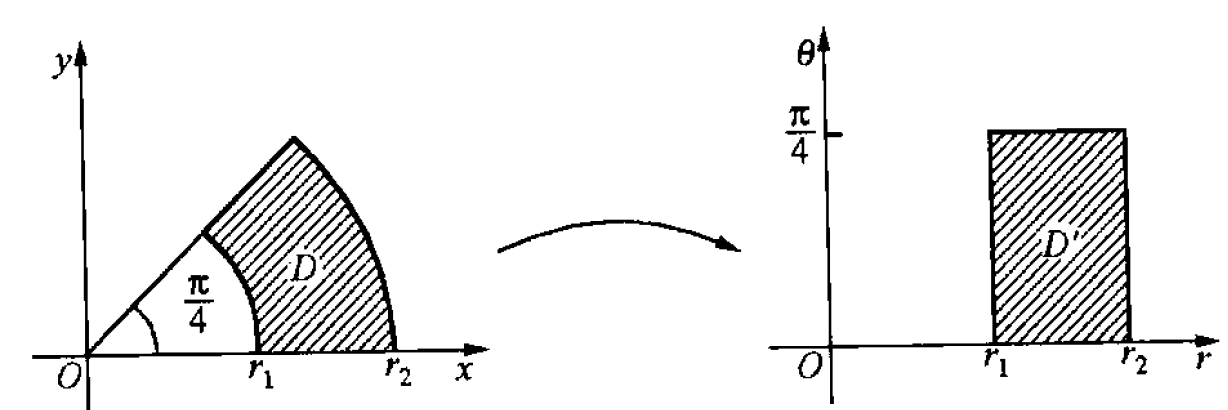
\includegraphics[scale=0.4]{figures/non-linear transform.png}
	\caption{从平面极坐标系到笛卡尔坐标系}
\end{figure}
此外,上面这个例子也能说明,对于非线性变换,曲线可能会变成直线,直线可能会变成曲线。\par   

那么真实物理世界的参考系变换,就不应该是非线性变换。否则,加入我们还是按照上面这个例子,$K$ 系和 $K'$ 系之间的坐标变换是这样的一个非线性变换
\begin{equation}
	\left\{\begin{aligned}
		x&=x'\cos y' \\
		y&=x'\sin y'
	\end{aligned}\right.
\end{equation}
那么原本在 $K$ 系中的“电子在匀强磁场中做匀速圆周运动”的规律可能在 $K'$ 系中就变成了匀速直线运动。

综上所述,考虑时空的均匀性,不同惯性系之间的变换应当为线性变换。所以洛伦兹变换应当是线性变换,可以用一个矩阵表示,记为$\Lambda(|\vb*{v}|)$,注意它只与速度的大小$|\vb*{v}|$有关,与方向无关,因而不能写成$\Lambda(\vb*{v})$. 接下来我们要说明三件事:
\begin{itemize}
	\item 对于洛伦兹标量,洛伦兹变换为 $S'=S$
	\item 对于洛伦兹向量,洛伦兹变换为 $A'^{\mu}=\Lambda^{\mu}_{\nu}A^{\nu}$
	\item 对于洛伦兹张量,洛伦兹变换为 $T'^{\mu\nu}=\Lambda^{\mu}_{\alpha}\Lambda^{\nu}_{\beta}T^{\alpha\beta}$
\end{itemize}

\section{洛伦兹变换}

\subsection{间隔不变性}

首先,我们证明\textbf{时空间隔在不同参考系下是不变的。}什么是时空间隔?那就是两个事件在四维时空中的“间距”呗。这样说太笼统,能不能给出一个确切的定义?
当然可以,下文就有。但后面会提到这个定义是怎么来的,下面的推导不需要用到其形式。\par   

假如在参考系$K$中有两个事件:$(t_{1},\vb*{x}_{1})$和$(t_{2},\vb*{x}_{2})$,它们之间的时空间隔为 $\Delta s^{2}\equiv c^{2}\Delta t^{2}-\Delta\vb*{x}^{2}$.
那么对于另一参考系$K'$,假定在$K$系看来它以速度$\vb*{v}$运动。
在$K'$系下,两事件被描述为:$(t_{1}',\vb*{x'}_{1})$和$(t'_{2},\vb*{x}'_{2})$,
由光速不变原理,在 $K'$ 系中这两个事件的时空间隔为 $\Delta s'=c^{2}\Delta t'^{2}-\vb*{x'}^{2}$. 由洛伦兹变换,结合运动的相对性
\begin{equation}
	\Delta s^{2}=\Lambda(|\vb*{v}|)\Delta s'^{2},\quad \Delta s'^{2}=\Lambda(|-\vb*{v}|)\Delta s^{2}
\end{equation}
显然,$\Lambda(|\vb*{v}|)$是一个常数,且$\Lambda^{2}=1$;再由变换的连续性,知 $\Lambda=1$.这样我们就证明了,时空间隔是不变的,即
\begin{equation}
	\Delta s'^{2}=\Delta s^{2}
\end{equation}

\subsection{洛伦兹标量}

我们将保持时空间隔不变的线性变换称为洛伦兹变换,在洛伦兹变换下保持不变的量称为洛伦兹标量,常见的洛伦兹标量有
\begin{itemize}
	\item 时空间隔:$\Delta s^{2}=c^{2}\Delta t^{2}-\Delta\vb*{x}^{2}$
	\item 四维体积元:$\dd[4]{x}$
	\item 静质量:$m_{0}$
	\item 固有时间:$\tau$
	\item 波的相位:$\phi=\omega t-\vb*{k}\cdot\vb*{x}$
\end{itemize}
其中$\dd[4]{x}$的含义我们后面会提到,它表示闵氏空间的体积微元;固有时间$\tau$的含义,形象地说其实就是相对于粒子静止的那个钟指示的时间;而其它物理量能成为洛伦兹标量,应当是容易理解的。比如粒子的静质量是粒子的内禀属性,不会随参考系的变化而改变;相位是一种客观存在,波峰波谷的数目是能够数出来的,自然也不会随着参考系发生任何变化。\par 

\subsection{洛伦兹变换的向量与矩阵形式}

对于惯性系$K$中任意一个事件$(t,x,y,z)$,它到原点的时空间隔的平方写为
\begin{equation}
	s^{2}=c^{2}t^{2}-x^{2}-y^{2}-z^{2}
\end{equation}
由于洛伦兹变换保持$s^{2}$不变,因而可以类比欧氏空间中的旋转也保持欧氏距离不变,将闵氏空间中的洛伦兹变换看成闵氏空间的一个“转动”。如果单纯考虑$x-t$平面的转动,那么需要保持 $c^{2}t^{2}-x^{2}=c^{2}t'^{2}-x'^{2}$,高中数学训练让我们联想到朴实无华的平方差公式,也就是写成$(ct'+x')(ct'-x')=(ct+x)(ct-x)$的形式,那么我们可以考虑如下变换
\begin{equation}
	\left\{\begin{aligned}
		ct'+x'&=\mathrm{e}^{\phi}(ct+x)\\
		ct'-x'&=\mathrm{e}^{-\phi}(ct-x)
	\end{aligned}\right.
\end{equation}
化简上式,很容易就出现了双曲三角函数,定睛一看,诶?下式是不是很像欧氏空间的旋转呢?只不过咱们把三角函数换成了双曲三角函数(这个咱们后面细聊)
\begin{equation}
	\left\{\begin{aligned}
		x'&=x\cosh\phi+ct\sinh\phi\\
		ct'&=x\sinh\phi+ct\cosh\phi
	\end{aligned}\right.\Leftrightarrow
	\begin{pmatrix}
		x' \\ ct'
	\end{pmatrix}=
	\begin{pmatrix}
		\cosh\phi & \sinh\phi \\
		\sinh\phi & \cosh\phi
	\end{pmatrix}
	\begin{pmatrix}
		x \\ ct
	\end{pmatrix}
\end{equation}
现在我们已经写出来了变换矩阵,这其实就是一个很大的成果了。考虑到$\cosh^{2}\phi-\sinh^{2}\phi=1$,我们可以在变换的框架下重新验证一下这种变换确实能保持时空间隔不变
\begin{equation}\begin{split}
	s'^{2}&=(x',ct')\begin{pmatrix}-x'\\ct'\end{pmatrix}\\
	&=
	(x,ct)
	\begin{pmatrix}
		\cosh\phi & \sinh\phi \\
		\sinh\phi & \cosh\phi
	\end{pmatrix}
	\begin{pmatrix}
		\cosh\phi & -\sinh\phi \\
		-\sinh\phi & \cosh\phi
	\end{pmatrix}\begin{pmatrix}-x\\ct\end{pmatrix}\\
	&=(x,ct)\begin{pmatrix}
		1 & 0 \\
		0 & 1
	\end{pmatrix}
	\begin{pmatrix}-x'\\ct'\end{pmatrix}\\
	&=s^{2}
\end{split}\end{equation}
上述计算过程需要注意两点:一是矩阵的转置规则,如$(AB)^{T}=B^{T}A^{T}$,如果不熟练的话我给你提个醒;
二是对于$(-x,ct)^{T}$,它的变换矩阵要做对应的调整,但这个我前面没有提到。
之后就是求这个“旋转角”了,我们后面会叫它“双曲角”,故意用 $\phi$ 而不是 $\theta$,就是想要区分“圆周角”。
那么这个双曲角怎么求呢?其实挺简单的,只需要在$K$系中考察$K'$原点的运动轨迹,类比一下,立马知道$\tanh\phi=\beta\equiv\dfrac{v}{c}$,所以就得到了式\eqref{e1}.\par   
\begin{figure}[H]
	\centering
	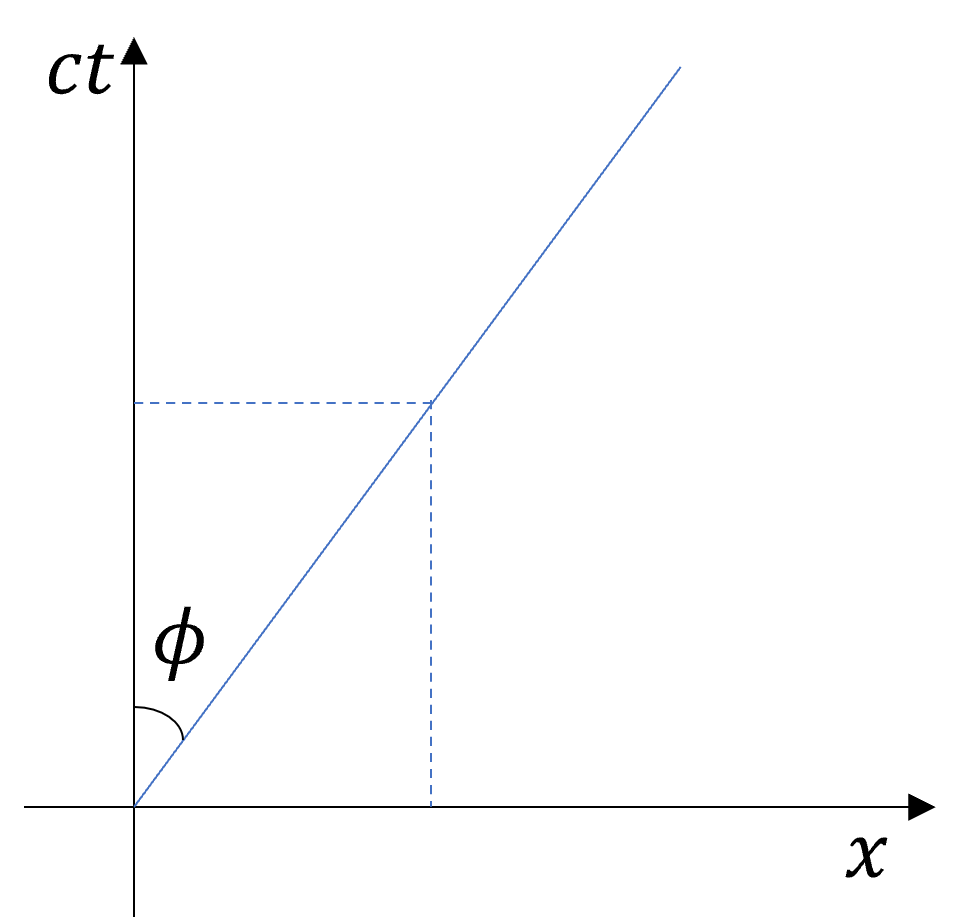
\includegraphics[scale=0.5]{figures/tanh_phi.png}
	\caption{$K'$系原点在$K$系中的轨迹}
\end{figure}
我当然希望读者能理解上述方法,但其中双曲角的求解,带一点“类比”、“不严谨”的色彩,后面会细聊。当然,实在不行,我们也完全可以使用待定系数法,把这个矩阵的$4\times4=16$个分量都设出来,依次求解。\par 
如果$K'$系相对于$K$系的速度是任意的,换句话说我们考虑闵氏空间的任意一个转动,那么式\eqref{e1}的推广也是很显然的,沿着方向$\vb*{\beta}$,将向量$\vb*{x}$正交分解,得到(有没有发现下述求平行分量的操作其实就是施密特正交化方法呢!)
\begin{equation}
	\vb*{x}_{\parallel}=|\vb*{x}|\cos\left<\vb*{x},\vb*{\beta}\right>\dfrac{\vb*{\beta}}{|\vb*{\beta}|}=\dfrac{\vb*{x}\cdot\vb*{\beta}}{\vb*{\beta}^{2}}\vb*{\beta},\quad\vb*{x}_{\perp}=\vb*{x}-\dfrac{\vb*{x}\cdot\vb*{\beta}}{\vb*{\beta}^{2}}\vb*{\beta}
\end{equation}
然后对平行分量和垂直分量依次代入式\eqref{e1},得到
\begin{equation}\label{e1.11}
	ct'=\gamma(ct-\vb*{\beta}\cdot\vb*{x}),\quad \vb*{x}'=\vb*{x}+\dfrac{\gamma-1}{\vb*{\beta}^{2}}(\vb*{\beta}\cdot\vb*{x})\vb*{\beta}-\gamma\vb*{\beta}ct
\end{equation}
这个结果很重要,已经很接近那个优美的结果了,就是类比牛顿第二定律的那种优美,但稍安勿躁,我们再做一丢丢铺垫。前面提到了闵氏时空却没有过多解释,只知道它是一个四维空间,这里给出闵氏时空中任一点的坐标,其各个分量依次定义为(下面的上标都不是幂次,而是指标,注意根据语境来区分)
\begin{equation}
	x^{0}=ct,x^{1}=x,x^{2}=y,x^{3}=z
\end{equation}
将指标统一记为$\mu$,其中$\mu=0,1,2,3$,那么闵氏空间中的任一向量可以写为
\begin{equation}
	x^{\mu}=(ct,\vb*{x})
\end{equation}
我们将这种闵氏空间中的矢量称为4-矢量,并且人为规定了指标在上和在下这两种情况,称$x^{\mu}$为逆变4-矢量,称$x_{\mu}$为协变4-矢量,其中
\begin{equation}
	x_{\mu}=(ct,-\vb*{x})
\end{equation}
这样定义后,显然就能直接用我们熟悉的向量内积来计算时空间隔,即
\begin{equation}
	s^{2}=x_{\mu}x^{\mu}=c^{2}t^{2}-\vb*{x}^{2}
\end{equation}
以上符号如果没弄明白的话,我再解释一下:$x^{\mu}$表示一个4-矢量,其上标$\mu$只是表示它是逆变矢量,而不要误会成$x^{\mu}$是4-矢量的某一个分量——拿三维欧氏空间中的向量$\vb*{v}$来举例,$v_{x}$或者$v_{1}$表示的是向量$\vb*{v}$的第一个分量,而表示向量本身。同样呢,$x_{\mu}$表示一个协变4-矢量,而不是表示某个分量,它就是矢量本身。另外,矢量乘法$x_{\mu}x^{\mu}$在这里称为指标的缩并,其实类似爱因斯坦求和约定,只是这里$x_{\mu}$不表示某一分量,并且指标的缩并一定是成对进行的,即一个上指标一个下指标。这个规定在4-矢量这里不太感觉得到,到4-张量那里会察觉到的。\par 
好了,定义了4-矢量后,我们结合式\eqref{e1.11},发现它可以用逆变4-矢量写为
\begin{equation}\label{e1.16}
	x'^{\mu}=\Lambda^{\mu}_{\nu}x^{\nu}
\end{equation}
其中$\Lambda^{\mu}_{\nu}$是一个张量,其矩阵表达式可以对照着写出来,具体为
\begin{equation}
	\Lambda(\vb*{\beta})=\begin{pmatrix}
		\gamma & -\gamma\beta_{1} & -\gamma\beta_{2} & -\gamma\beta_{3} \\
		-\gamma\beta_{1} & 1+(\gamma-1)\dfrac{\beta_{1}^{2}}{\vb*{\beta}^{2}} & (\gamma-1)\dfrac{\beta_{1}\beta_{2}}{\vb*{\beta}^{2}} & (\gamma-1)\dfrac{\beta_{1}\beta_{3}}{\vb*{\beta}^{2}} \\
		-\gamma\beta_{2} & (\gamma-1)\dfrac{\beta_{2}\beta_{1}}{\vb*{\beta}^{2}} & 1+(\gamma-1)\dfrac{\beta_{2}^{2}}{\vb*{\beta}^{2}} & (\gamma-1)\dfrac{\beta_{2}\beta_{3}}{\vb*{\beta}^{2}} \\
		-\gamma\beta_{3} & (\gamma-1)\dfrac{\beta_{3}\beta_{1}}{\vb*{\beta}^{2}} & (\gamma-1)\dfrac{\beta_{3}\beta_{2}}{\vb*{\beta}^{2}} & 1+(\gamma-1)\dfrac{\beta_{3}^{2}}{\vb*{\beta}^{2}}
	\end{pmatrix}
\end{equation}
看式\eqref{e1.16},仔细体会其中的指标缩并法则,尤其是涉及到张量到$\Lambda_{\nu}^{\mu}$的情况该如何缩并。\par 

\subsection{洛伦兹矢量}

好了,我们已经得到一个真正意义上的、形式完整的洛伦兹变换了!从变换的角度,我们将像逆变4-矢量$x^{\mu}$这种符合洛伦兹变换的物理量称为洛伦兹矢量,并且洛伦兹矢量的内积就是洛伦兹标量。洛伦兹矢量还有很多,比如
\begin{itemize}
	\item 4-速度:$U^{\mu}=(\gamma c,\gamma\vb*{v})$
	\item 4-动量:$P^{\mu}=\qty(\dfrac{E}{c},\vb*{p})$
	\item 4-力:$F^{\mu}=\qty(\dv{P^{0}}{\tau},\dv{\vb*{p}}{\tau})$
	\item 4-加速度:$A^{\mu}=\dv{U^{\mu}}{\tau}=(\dv{\gamma}{\tau}c+\gamma\dv{\vb*{v}}{\tau},\gamma\dv{\vb*{a}}{\tau})$
	\item 4-电流密度:$J^{\mu}=(\rho c,\vb*{j})$
	\item 4-波矢:$k^{\mu}=\qty(\dfrac{\omega}{c},\vb*{k})$
\end{itemize}
后面会发现狭义相对论的技术性结论基本上都能从这个优美的洛伦兹变换中推导出来,所以弄清楚洛伦兹矢量是非常重要的。我们现在就来弄清楚这几个4-矢量,以及前面我们没有搞懂的两个4-标量,究竟是怎么来的。

\subsection{固有时和坐标时}

首先,闵氏时空下最基本的坐标微元是$\dd{x^{\mu}}=(c\dd{t},\dd{\vb*{x}})$,显然,4-矢量的内积都是洛伦兹标量,于是我们知道
\begin{equation}\label{e1.18}
	\dd{\tau^{2}}\equiv\dfrac{1}{c^{2}}\dd{x_{\mu}}\dd{x^{\mu}}
\end{equation}
一定是一个洛伦兹标量,它就是前面提到的固有时的定义。我们提到它的含义是粒子携带的那个钟指示的时间,那么我们就以粒子为参考系,那么有$\dd{x^{\mu}}=(c\dd{t},0,0,0)$,此时就有$\dd{\tau}=\dd{t}$,现在这个含固有时间的物理含义解释清楚了吧。而一般情况下,根据式\eqref{e1.18},我们可以计算得到
\begin{equation}\label{e1.19}
	\dd{\tau}=\dfrac{\dd{t}}{\gamma}
\end{equation}
显然,当且仅当$\gamma=1$时,$\dd{\tau}=\dd{t}$,而$\gamma=1$也就意味着粒子的速度$\vb*{v}=0$.式\eqref{e1.19}是不是很自然地就得到了“钟慢”效应?因为质点一旦运动,就有$\gamma>1$,就有$\dd{\tau}<\dd{t}$,也就是我们经常说的质点携带的钟“走的更慢”。\par 

\subsection{四维速度}

接下来,我们考察4-速度,其定义其实就是速度$\vb*{v}=\dv{\vb*{x}}{t}$在闵氏时空的简单推广:
\begin{equation}
	U^{\mu}\equiv\dv{x^{\mu}}{\tau}=(\gamma c,\gamma\vb*{v})
\end{equation}
为什么是对$\tau$微分呢?因为它是4-标量诶,现在感受到这个定义的自然了吧。这里需要提一下,这个$U^{\mu}$的四维长度为
\begin{equation}
	\sqrt{U_{\mu}U^{\mu}}=c
\end{equation}
虽然$U^{\mu}$的定义比较自然,但是它的含义却远不如$\vb*{v}$清晰。我当前的理解是,在我们没有进行闵氏时空的深入讨论之前,不需要太着重探讨$U^{\mu}$的物理含义,只需要知道它是一个洛伦兹矢量,满足洛伦兹变换,能够求出速度变换公式。现假设一质点在$K$系的速度为$\vb*{v}=(v_{x},v_{y},v_{z})$,而另一惯性系$K'$相对$K$系以速度$\vb*{u}$运动,我们希望求出该质点在$K'$系中的速度$\vb*{v}'$。利用4-速度的洛伦兹变换,有
\begin{equation}
	U'^{\mu}=\Lambda^{\mu}_{\nu}U^{\nu}
\end{equation}
其中$U^{\mu}=(\gamma_{\vb*{v}} c,\gamma_{\vb*{v}}\vb*{v})$,$U'^{\mu}=(\gamma_{\vb*{v}'} c,\gamma_{\vb*{v}'}\vb*{v}')$,而变换矩阵$\Lambda^{\mu}_{\nu}$中$\gamma=\dfrac{1}{\sqrt{1-u^{2}/c^{2}}}$.依据式\eqref{e1.11}可以得到
\begin{equation}
	\begin{split}
		\vb*{v}'&=\dv{\vb*{x}'}{t'}\\
		&=\dfrac{\dd{\vb*{x}}+(\gamma-1)\dfrac{\vb*{u}\cdot\dd{\vb*{x}}}{\vb*{u}^{2}}\vb*{u}-\gamma\vb*{u}\dd{t}}{\gamma\qty(\dd{t}-\dfrac{\vb*{u}\cdot\dd{\vb*{x}}}{c^{2}})}\\
		&=\dfrac{\vb*{v}+\qty[(\gamma-1)\dfrac{\vb*{u}\cdot\vb*{v}}{\vb*{u}^{2}}-\gamma]\vb*{u}}{\gamma\qty(1-\dfrac{\vb*{u}\cdot\vb*{v}}{c^{2}})}
	\end{split}
\end{equation}
若令$\vb*{u}=(u,0,0)$,则上式可具体展开为分量形式
\begin{equation}\label{general-velocity-superposition}
	v_{x}'=\dfrac{v_{x}-u}{1-\dfrac{uv_{x}}{c^{2}}},\quad v_{y}'=\dfrac{v_{y}}{\gamma\qty(1-\dfrac{uv_{x}}{c^{2}})},\quad v_{z}'=\dfrac{v_{z}}{\gamma\qty(1-\dfrac{uv_{x}}{c^{2}})}
\end{equation}

\subsection{四维动量}

利用4-速度,我们可以进一步很自然地定义4-动量
\begin{equation}
	P^{\mu}\equiv m_{0}U^{\mu}=(\gamma m_{0}c,\gamma m_{0}\vb*{v})
\end{equation}
其中需要讨论一下$P^{0}$,它与质点的能量有关,在$v\ll c$时用泰勒展开
\begin{equation}
	P^{0}=\gamma m_{0}c=\dfrac{m_{0}c}{\sqrt{1-\dfrac{v^{2}}{c^{2}}}}=\dfrac{1}{c}\qty(m_{0}c^{2}+\dfrac{1}{2}m_{0}v^{2}+\cdots)
\end{equation}
显然这第二项是物体的动能,这就是为何我们说$P^{0}$与能量有关。现在设闵氏空间中质点的能量为
\begin{equation}
	E\equiv\gamma m_{0}c^{2}
\end{equation}
那么4-动量可进一步改写为
\begin{equation}
	P^{\mu}=\qty(\dfrac{E}{c},\gamma m_{0}\vb*{v})=\qty(\dfrac{E}{c},\vb*{p})
\end{equation}
我们发现当质点静止时,$P^{\mu}=(m_{0}c,0,0,0)$,也就是说此时粒子还是具有一定的能量,我们称之为静止能量
\begin{equation}
	E_{0}\equiv m_{0}c^{2}
\end{equation}
那显然,闵氏空间中质点的动能就写为
\begin{equation}
	T=(\gamma-1)m_{0}c^{2}
\end{equation}
起初可能会觉得在能量中加一个常数项$E_{0}$很奇怪,是不是可以删去?第一,由于协变性的要求,质点的静止能量这一项必须存在,不可或缺。第二,在核反应中,我们已经发现粒子的静止能量能转化为动能,也就是说这部分能量是有实际的物理意义的。所以,它不仅不能删去,而且还揭示了著名的质能关系。最后我们计算4-动量的四维长度
\begin{equation}
	\sqrt{P_{\mu}P^{\mu}}=m_{0}c
\end{equation}
这给出来一条重要结论,也就是我们常说的相对论性能量动量关系
\begin{equation}
	E=\sqrt{\vb*{p}^{2}c^{2}+m_{0}^{2}c^{4}}
\end{equation}

\subsection{四维力}

现在,我们来讨论4-力,引入了4-动量后,很自然就给出来4-力的定义
\begin{equation}\label{e1.33}
	F^{\mu}\equiv\dv{P^{\mu}}{\tau}=\qty(\dfrac{P}{c},\gamma\vb*{F})
\end{equation}
这显然也是一个洛伦兹矢量,其中$F^{0}$与$\vb*{F}$的关系如下
\begin{equation}
	\begin{split}
		F^{0}&=\dv{P^{0}}{\tau}\\
		&=\dfrac{1}{c}\dv{\tau}\sqrt{\vb*{p}^{2}c^{2}+m_{0}c^{4}}\\
		&=\dfrac{1}{c}\dfrac{c^{2}}{E}\vb*{p}\cdot\dv{\vb*{p}}{\tau}\\
		&=\dfrac{1}{c}\vb*{v}\cdot\dv{\vb*{p}}{\tau}\\
		&=\dfrac{\gamma}{c}\vb*{F}\cdot\vb*{v}
	\end{split}
\end{equation}
显然它表示功率,所以在式\eqref{e1.33}中我们用了$P=\vb*{F}\cdot\vb*{v}$的这种常用标记。另外,在上面的过程中,我们也悄悄定义了$\vb*{F}$
\begin{equation}
	\vb*{F}\equiv\dv{\vb*{p}}{t}
\end{equation}
其实就是相对论力学方程,它表明力$\vb*{F}$等于动量变化率,力$\vb*{F}$做的功等于能量变化率。



\chapter{几何直观}

按照我个人的习惯,前面的那些推导能弄懂的话,考试就能应付得来;但真正给别人讲知识本身的时候,除非你有几何直观的理解,否则很难讲清楚。
这一章,就是几何直观:关于洛伦兹变换的几何直观,关于闵氏时空的几何直观,关于狭义相对论能解决的经典悖论的几何直观。
此外,通过这一部分把前面洛伦兹矩阵的推导过程中“类比”出来的东西严格化,比如时空间隔的定义,比如双曲角的求解。\par   

\section{从速度叠加公式说起}

我们先考虑一个问题:
$K'$ 系的原点在 $K$ 系中的速度为 $u$,而一个质点在 $K'$ 系中的速度为 $v'$,求它在 $K$ 系中的速度 $v$。\par   
答案是咱们熟知的速度叠加公式,一般的情形在前面\eqref{general-velocity-superposition}提到了,对于咱们一维情形,速度叠加后为
\begin{equation}
	v=\frac{u+v'}{1+\frac{uv'}{c^{2}}}
\end{equation}
这个答案有点复杂,没有伽利略变换那样 $v=u+v'$ 直接叠加来得自然。但无论如何,咱们还是得好好端详这个结论,然后给它记住。虽说要记住,不过还是觉得不服,因为这个叠加公式真的不太直观。\par   
Wait! 有没有觉得这个公式的形式,有点眼熟?回忆一下,好像跟正切函数的和角公式有点像:
\begin{equation}
	\tan(\theta_{1}+\theta_{2})=\frac{\tan\theta_{1}+\tan\theta_{2}}{1-\tan\theta_{1}\tan\theta_{2}}
\end{equation}
比较像,但是有两个不同:一是分母的加减号不一样,二是分母多了个系数。系数无大所谓,符号更要命些。为啥呢,咱们可以这样操作:
\begin{equation}\label{adjusted-1D-velocity-superposition}
	\frac{v}{c}=\frac{\frac{u}{c}+\frac{v'}{c}}{1+\frac{u}{c}\frac{v'}{c}}
\end{equation}
这时候 $v/c$ 就和 $\tan(\theta_{1}+\theta_{2})$ 几乎就能对应了,这也意味着在狭义相对论中,或许相比于 $v$ 叠加,$\beta$ 叠加更合适一点——但是还有个要命的符号问题。 \par 
那再想想,如果我们考虑它的近亲,双曲正切函数呢?
\begin{equation}\label{hyperbolic-tangent's-additon-formula}
	\tanh(\phi_{1}+\phi_{2})=\frac{\tanh\phi_{1}+\tanh\phi_{2}}{1+\tanh\phi_{1}\tanh\phi_{2}}
\end{equation}
你别说,这回真挺像了,简直是一模一样!两个公式的结构完全,那么它们一定有内在的联系,抓住这条线索,应该就能让狭义相对论下的速度叠加变得容易理解!\par   
对照\eqref{adjusted-1D-velocity-superposition}和\eqref{hyperbolic-tangent's-additon-formula},我们可以发现,$\beta$ 和 $\tanh(\phi_{1}+\phi_{2})$ 是完全对应的。那么我们就有底气宣称:在狭义相对论中,相比于 $\beta$ 叠加,$\phi$ 叠加才是本质。\par   
Wait! 这个 $\phi$ 是什么?跟 $\theta$ 一样是角度嘛?不是,显然不是。那它是某种几何量吗?可以是,如果我们接受双曲几何,那么 $\phi$ 就是双曲角。\par   
这就像是第一道刺破黑夜的曙光,现在,我们对速度叠加公式的几何理解终于有希望了。


\section{双曲几何}

这里通过类比的方式来介绍双曲几何的一些概念,从双曲角到双曲三角函数,再到距离,浅尝辄止。本节中,$\phi$ 表示双曲角,$\theta$ 表示圆周角。

\begin{figure}[H]
	\centering
	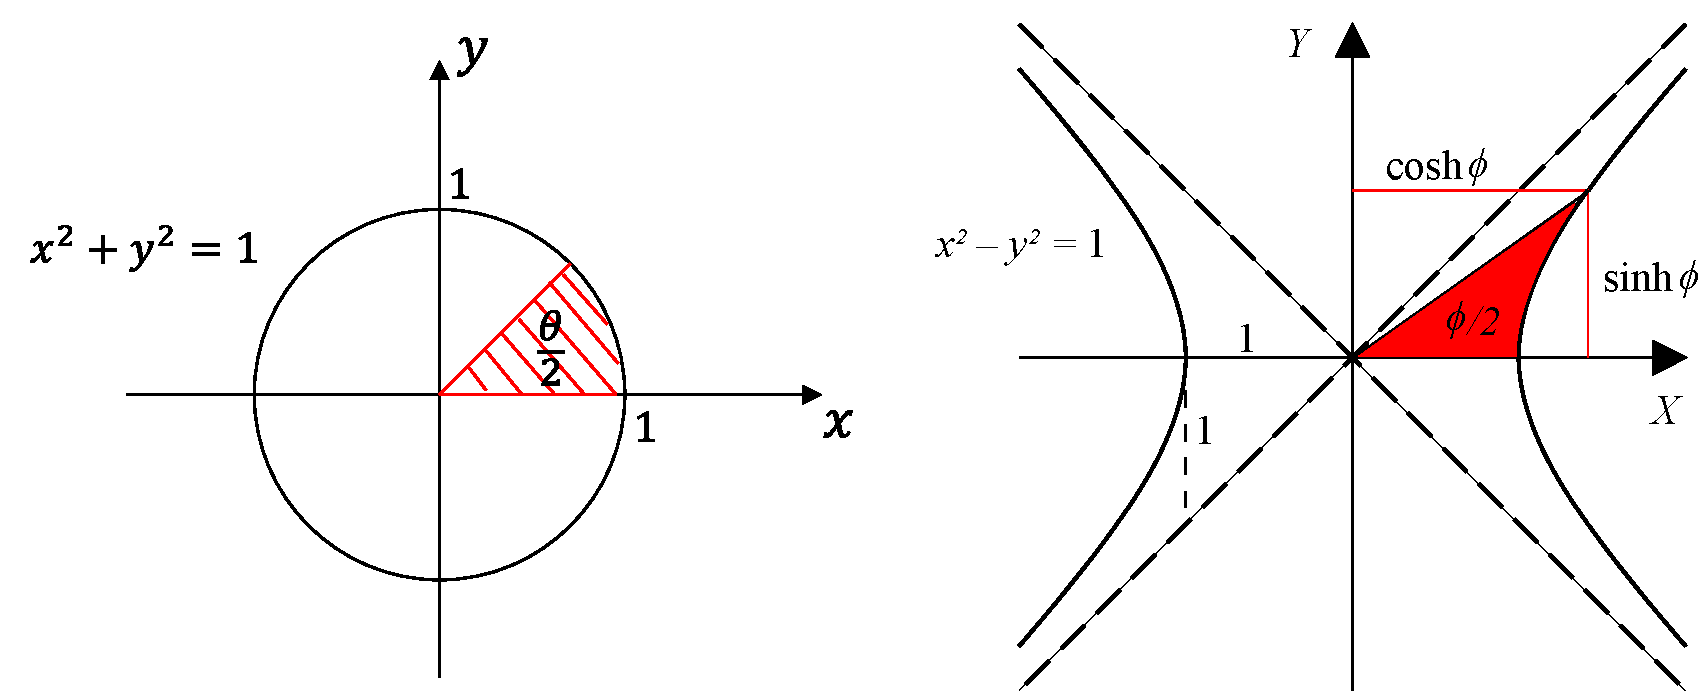
\includegraphics[scale=0.4]{figures/hyperbolic_function.pdf}
	\caption{圆周角和双曲角的几何含义}
\end{figure}

用类比的方法去理解双曲角。它和欧式几何中的圆周角一样,表示角度吗?显然不是,如果是角度的话,那么图中的双曲三角函数就应该替换为三角函数,但是显然不能替换,因为我们研究的双曲线是固定的,因而曲线上点的坐标之间的关系也随即确定了下来。\par   
\begin{equation}
	\left\{
	\begin{aligned}
		(x,y)\in C^{0}:x^{2}+y^{2}=1&\Rightarrow(x,y)\simeq(\cos\theta,\sin\theta)\\
		(x,y)\in C^{-}:x^{2}-y^{2}=1&\Rightarrow(x,y)\simeq(\cosh\phi,\sin\phi)
	\end{aligned}
	\right.
\end{equation}
那么,由于 $\theta$ 还能表示圆周上的弧长,难道 $\phi$ 也能表示双曲线上的弧长?
\begin{equation}
	\begin{aligned}
		s&=\int_{O}^{P}\dd{s}=\int_{O}^{P}\sqrt{\dd{x}^{2}+\dd{y}^{2}}\\
		&=\int_{0}^{\phi}\sqrt{\qty(\dv{x}{\phi})^{2}+\qty(\dv{y}{\phi})^{2}}\dd{\phi}\\
		&=\int_{0}^{\phi}\sqrt{\sinh^{2}\phi+\cosh^{2}\phi}\dd{\phi}>\phi_{P}
	\end{aligned}
\end{equation}
经过计算发现,也不是。\par   
再想想。$\theta$ 还能表示扇形面积的2倍,那么 $\phi$ 会不会也是双曲三角形面积的2倍呢?关于面积的计算,利用格林公式
\begin{equation}
	\oint\qty(P\dd{x}+Q\dd{y})=\oiint\qty(\pdv{Q}{x}-\pdv{P}{y})\dd{x}\dd{y}
\end{equation}
我希望将二重积分转化为线积分,那就需要让 $\pdv{Q}{x}-\pdv{P}{y}=1$,那么可以令 $P(x,y)=-\frac{y}{2},Q(x,y)=\frac{x}{2}$,那么
\begin{equation}
	\begin{aligned}
		S=&\frac{1}{2}\oint\qty(x\dd{y}-y\dd{x})\\
		&=\frac{1}{2}\int_{0}^{\phi}\qty(\cosh^{2}\phi-\sinh^{2}\phi)\\
		&=\frac{\phi}{2}
	\end{aligned}
\end{equation}
还真是!原来双曲角和圆周角的共同几何含义在于,它们都是对应圆周三角形或双曲三角形的面积!
\begin{figure}[H]
	\centering
	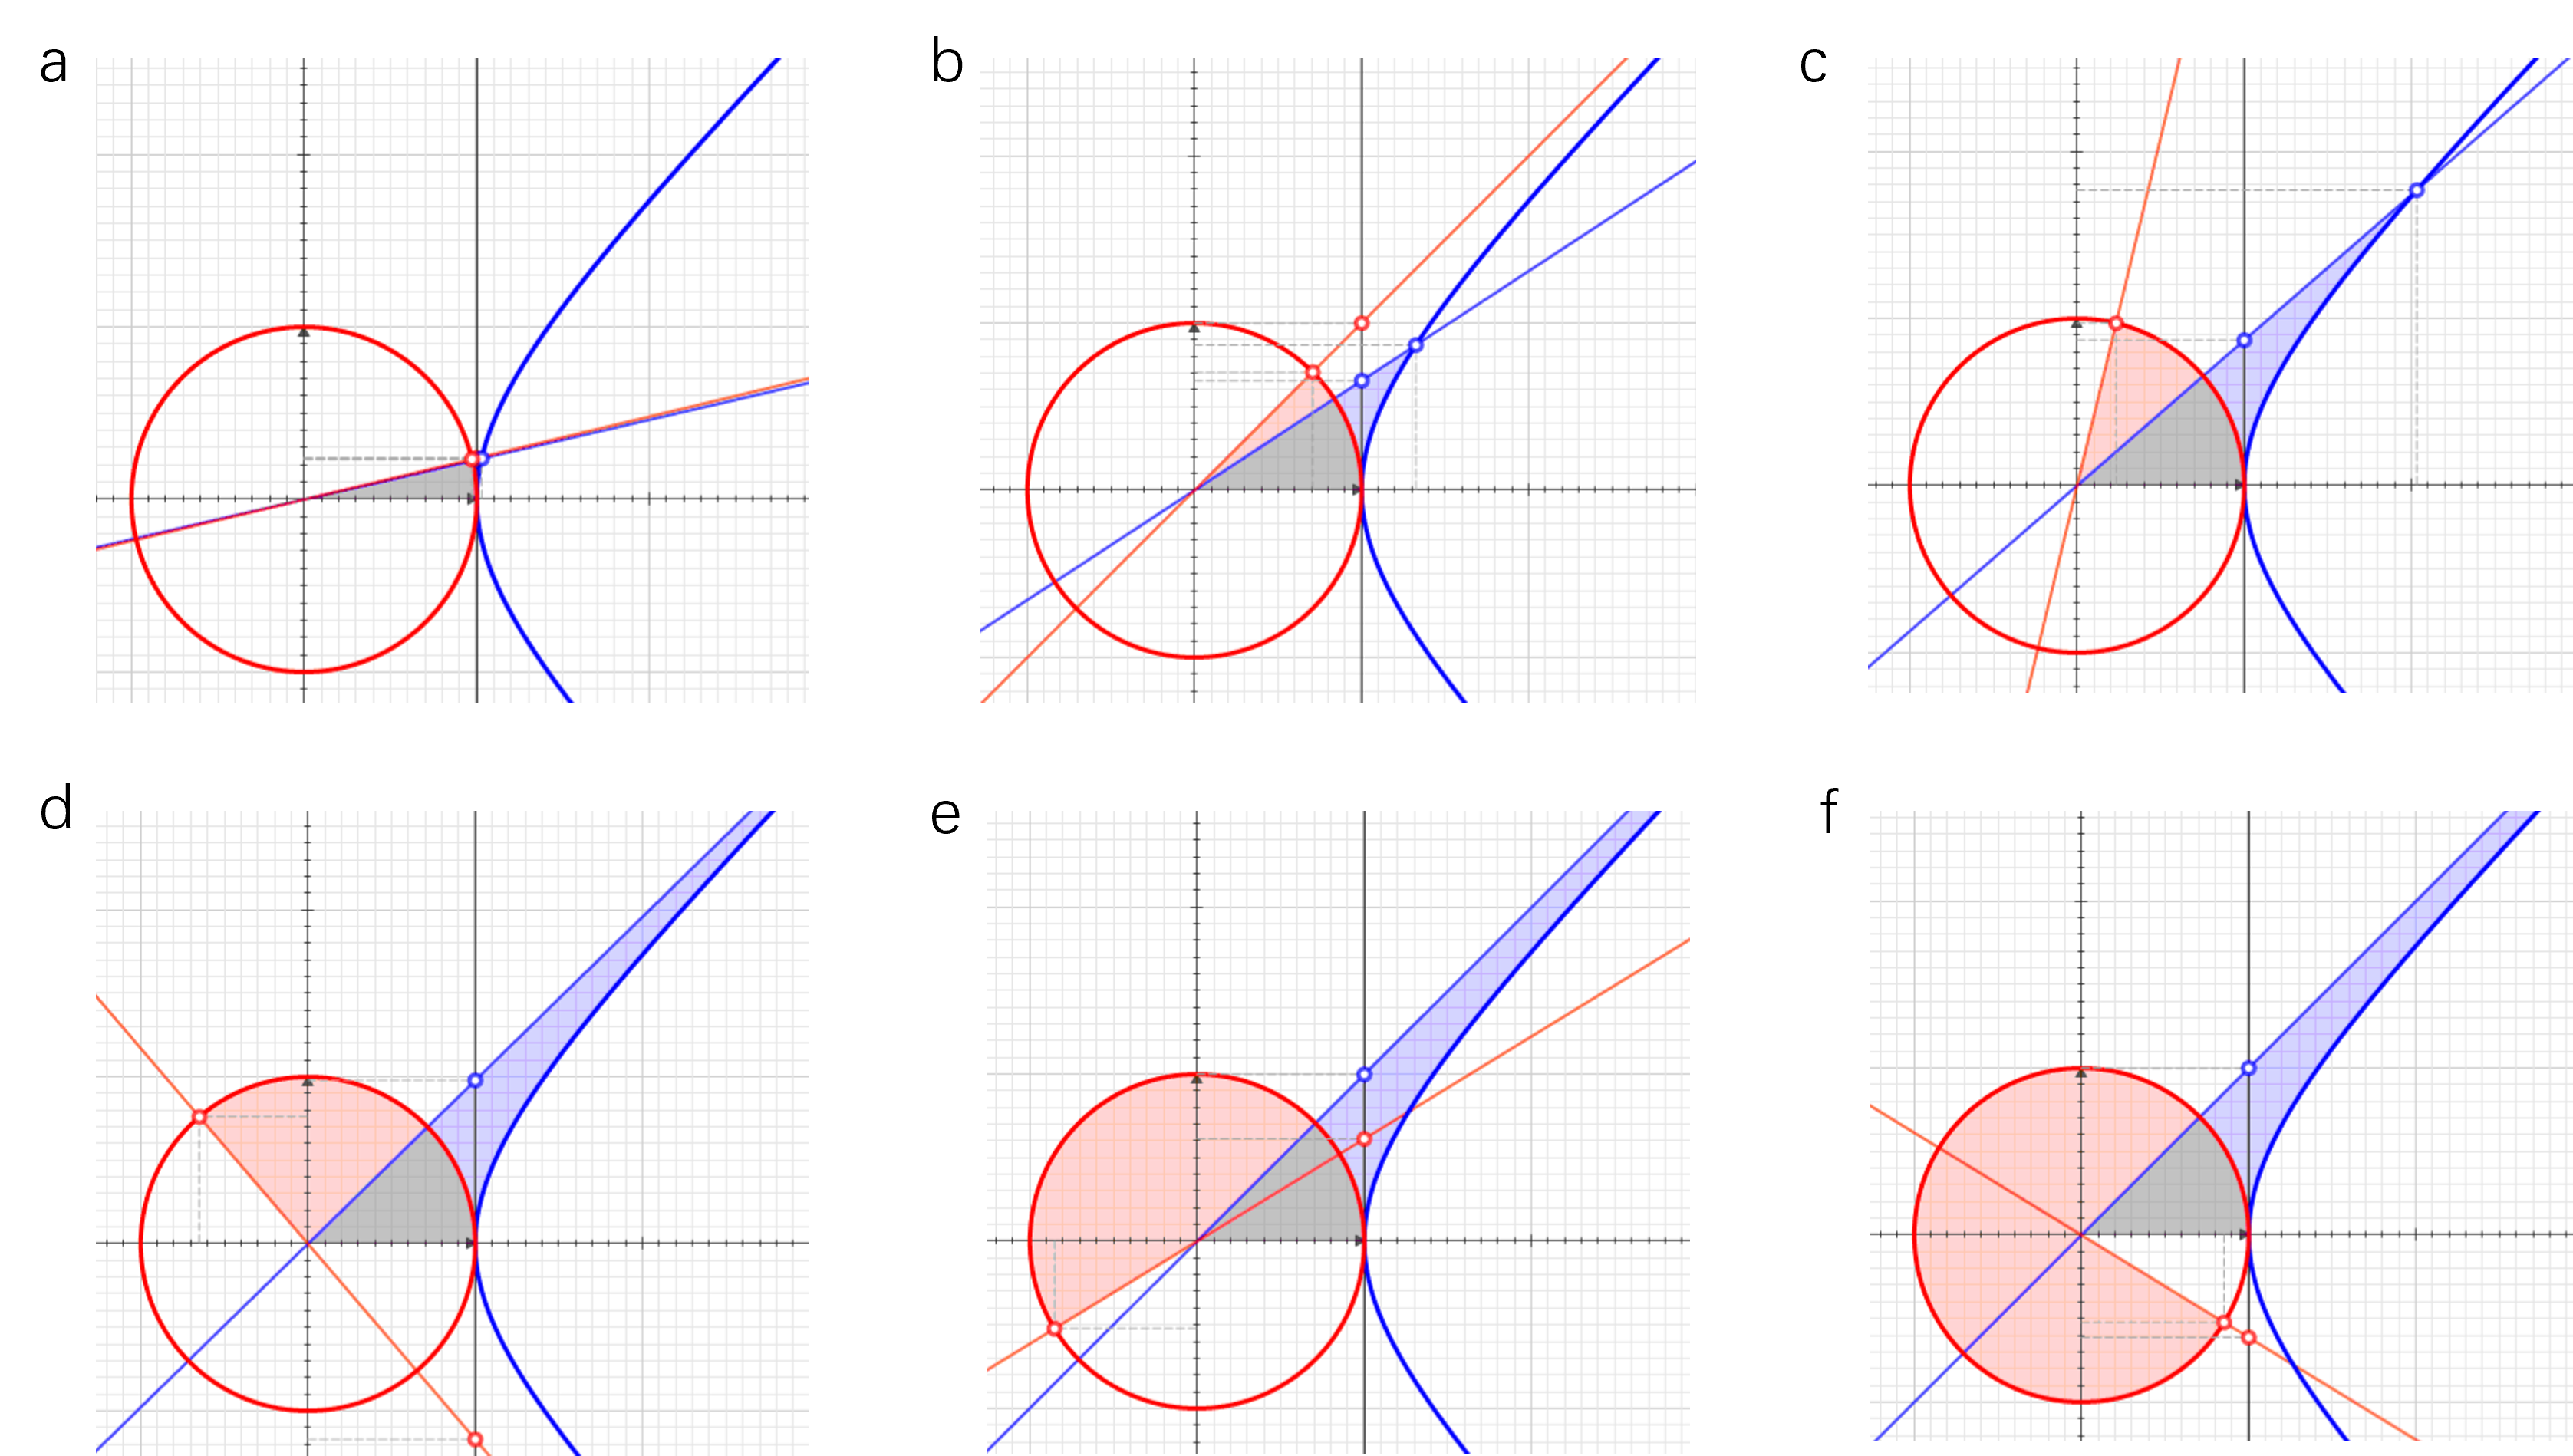
\includegraphics[scale=0.5]{figures/circular-hyperbolic-angle.png}
	\caption{圆周角和双曲角的变化范围}
\end{figure}
不过圆周角的变化是周期的,从0到$2\pi$,对应三角函数也是周期的;而双曲角的变化则不是周期的,从0到$+\infty$,对应双曲函数也不是周期的。\par   
此外,我们还可以看到,与 $\tan\theta$ 随着 $\theta$ 的变化会达到 $+\infty$ 不同,$\tanh\phi$ 永远小于1,它对应的是相对论时空中,$\beta<1$,或者说,质点的速度永远小于光速。\par   
除了双曲角,还有双曲距离可以讨论。在欧氏空间中,由于三角函数满足恒等式 $\sin^{2}\theta+\cos^{2}\theta=1$,欧氏距离很自然地定义为 $d^{2}=\Delta x^{2}+\Delta y^{2}$;在双曲空间中,同样由于双曲函数满足的恒等式 $\cosh^{2}\phi-\sinh^{2}\phi=1$,双曲距离定义为 $s^{2}=\Delta x^{2}-\Delta y^{2}$. 这不就是相对论时空中,时空间隔的定义嘛!\par   
在双曲几何的视角下,时空间隔、速度叠加、洛伦兹变换、尺缩钟慢等看似奇怪的现象都显得那么自然。事情都发展到这一步了,我们还有什么理由不去相信,狭义相对论的几何就是双曲几何呢!我们还有什么理由不去相信,狭义相对论的时空就是闵氏时空呢!\par   


\section{洛伦兹变换的几何直观}

既然狭义相对论的时空是闵氏时空,用到的几何是双曲几何,那么闵氏时空的坐标变换,也就是所谓的洛伦兹变换,应当可以利用双曲几何得到一个很好的几何直观。\par   
在进一步讨论之前,我们先简单梳理一下洛伦兹变换的有关内容: 
在闵氏时空中,我们将时空坐标定义成了逆变4-矢量 $x^{\mu}$ 和协变4-矢量 $x_{\mu}$,其中$x^{\mu}$的各个分量依次为
\begin{equation}
	x^{0}=ct,\ x^{1}=x,\ x^{2}=y,\ x^{3}=z
\end{equation}
而 $x_{\mu}$ 的空间分量要添加负号。\par   
之后我们推导出了同一个事件在 $K$ 系下的坐标 $x^{\mu}$ 和 $K'$ 系下的坐标 $x'^{\mu}$ 之间的,所谓洛伦兹变换
\begin{equation}
	x'^{\mu}=\Lambda^{\mu}_{\nu}x^{\nu}
\end{equation}
其中洛伦兹矩阵 $\Lambda_{nu}^{\mu}$ 是一个四维方阵,它与 $K$ 系下 $K'$ 的速度有关,其一般形式为
\begin{equation}
	\Lambda(\vb*{\beta})=\begin{pmatrix}
		\gamma & -\gamma\beta_{1} & -\gamma\beta_{2} & -\gamma\beta_{3} \\
		-\gamma\beta_{1} & 1+(\gamma-1)\dfrac{\beta_{1}^{2}}{\vb*{\beta}^{2}} & (\gamma-1)\dfrac{\beta_{1}\beta_{2}}{\vb*{\beta}^{2}} & (\gamma-1)\dfrac{\beta_{1}\beta_{3}}{\vb*{\beta}^{2}} \\
		-\gamma\beta_{2} & (\gamma-1)\dfrac{\beta_{2}\beta_{1}}{\vb*{\beta}^{2}} & 1+(\gamma-1)\dfrac{\beta_{2}^{2}}{\vb*{\beta}^{2}} & (\gamma-1)\dfrac{\beta_{2}\beta_{3}}{\vb*{\beta}^{2}} \\
		-\gamma\beta_{3} & (\gamma-1)\dfrac{\beta_{3}\beta_{1}}{\vb*{\beta}^{2}} & (\gamma-1)\dfrac{\beta_{3}\beta_{2}}{\vb*{\beta}^{2}} & 1+(\gamma-1)\dfrac{\beta_{3}^{2}}{\vb*{\beta}^{2}}
	\end{pmatrix}
\end{equation}
如果我们要寻找几何直观,最好还是只研究一维运动,此时洛伦兹变换为
\begin{equation}
	\begin{pmatrix}
		ct' \\ x'
	\end{pmatrix}=
	\begin{pmatrix}
		\gamma & -\gamma\beta \\
		-\gamma\beta & \gamma
	\end{pmatrix}\begin{pmatrix}
		ct \\ x
	\end{pmatrix}\Leftrightarrow
	\begin{pmatrix}
		ct' \\ -x'
	\end{pmatrix}=
	\begin{pmatrix}
		\gamma & \gamma\beta \\
		\gamma\beta & \gamma
	\end{pmatrix}\begin{pmatrix}
		ct \\ -x
	\end{pmatrix}
\end{equation}
到目前为止,变换的整体形式已经比较简单了,接下来我们要让它更简单。把上述公式放入双曲几何的框架中,我们惊奇地发现:
\begin{equation}
	\begin{pmatrix}
		\cosh\phi' \\ \sinh\phi'
	\end{pmatrix}=
	\begin{pmatrix}
		\cosh\phi_{0} & \sinh\phi_{0} \\
		\sinh\phi_{0} & \cosh\phi_{0}
	\end{pmatrix}\begin{pmatrix}
		\cosh\phi \\ \sinh\phi
	\end{pmatrix}=
	\begin{pmatrix}
		\cosh(\phi_{0}+\phi) \\ \sinh(\phi_{0}+\phi)
	\end{pmatrix}
\end{equation}
只要我们将时空坐标嵌入到双曲空间中,即 $(ct,-x)\simeq(\cosh\phi,\sinh\phi)$,那么几何含义也就一目了然了:\textbf{洛伦兹变换其实是双曲几何中的旋转。}  

\par 我举个例子,$K$ 系中 $K'$ 系的原点以速度 $v$ 运动,某一时刻两系的原点重合。此时,有一个事件,在 $K'$ 系中的时空坐标为 $(ct',x')$,那么如何求这个事件在 $K$ 系中的坐标呢?

\par 这个求解一方面可以用洛伦兹变换直接去计算,另一方面我们也可以用双曲几何的视角去看待问题:$K'$ 系的速度 $v=c\tanh\phi_{0}$,事件在 $K'$ 系中的坐标要变成协变形式 $(ct',-x')=(\cosh\phi',\sinh\phi')$,然后把这个 $\phi'$ 旋转 $\phi_{0}$,得到的就是 $K$ 系下的坐标在双曲几何中的双曲角 $\phi=\phi_{0}+\phi'$. 那么其协变形式就是 $(ct,x)=(\cosh(\phi_{0}+\phi'),\sinh(\phi_{0}+\phi'))$,如果需要的话再变为逆变形式 $(ct,x)$ 即可。

\par 当然了,既然是旋转,那是不是得有距离不变呢?当然,不管是 $(ct,x)$ 还是 $(ct',x')$,它到原点的距离都不变——别忘了,这个距离是双曲距离。


\section{悖论合集}

有些标题党了,其实这一部分除了解释所谓“悖论”以外,还要介绍许多比较经典的效应。

\subsection{尺缩钟慢,同时的相对性}

尺缩钟慢应该是狭义相对论最“出圈”的效应了吧。所谓“尺缩”,是指运动的物体看上去长度变短了;所谓“钟慢”,是指运动的物体他的固有钟走得变慢,这个“固有钟”是运动物体本身携带的钟,比如一个运动的人戴的腕表。

\par 我们不妨在表述的时候添加一些数学语言。将运动局限在一维直线运动中。观察者,也就是我们,位于 $K$ 系的原点。在 $K$ 系中,有一辆固有长度为 $l_{0}$ 的载具以速度 $u$ 直线运动。选取相对载具静止的参考系为 $K'$,并且让这两个参考系的原点重合。我们的问题是,在 $K$ 系中,载具的长度变为多少?载具上的钟走过单位时间,对应 $K$ 系中的钟走过了多久?

\par 根据前面的讨论,我们知道 $\dd{t}=\gamma\dd{\tau}$,这就是我们所说的钟慢;关于尺缩,我们用经典的洛伦兹变换去推导。设车头和车尾在 $K'$ 系中的时空坐标分别为 $(ct_{1}',x_{1}'),(ct_{2}',x_{2}')$,记这两个事件在 $K$ 系中的时空坐标为 $(ct_{1},x_{1}),(ct_{2},x_{2})$. 那么,
\begin{equation}
	l_{0}=x_{2}'-x_{1}',\quad\texttt{where}\quad t_{1}'-t_{2}'=0
\end{equation}
上式中的 $l_{0}$ 也叫固有长度,是在 $K'$ 系中同时测得车头、车尾的坐标得到的。那么用洛伦兹变换得到,
\begin{equation}
	l_{0}=x_{2}'-x_{1}'=\gamma\qty(\Delta x-\beta c\Delta t)
\end{equation}
想要在 $K$ 系中测量载具的长度,就需要在 $K$ 系中同时得到车头和车尾的坐标,即 $\Delta t=0$,那么自然得到
\begin{equation}
	l_{0}=\gamma l
\end{equation}
也就是说,在 $K$ 系看到的载具长度 $l$ 比它的固有长度 $l_{0}$ 要短。

\par 以上是典型的做法,我接下来会用几何的方法去建立直观理解。
\begin{figure}[H]
	\centering
	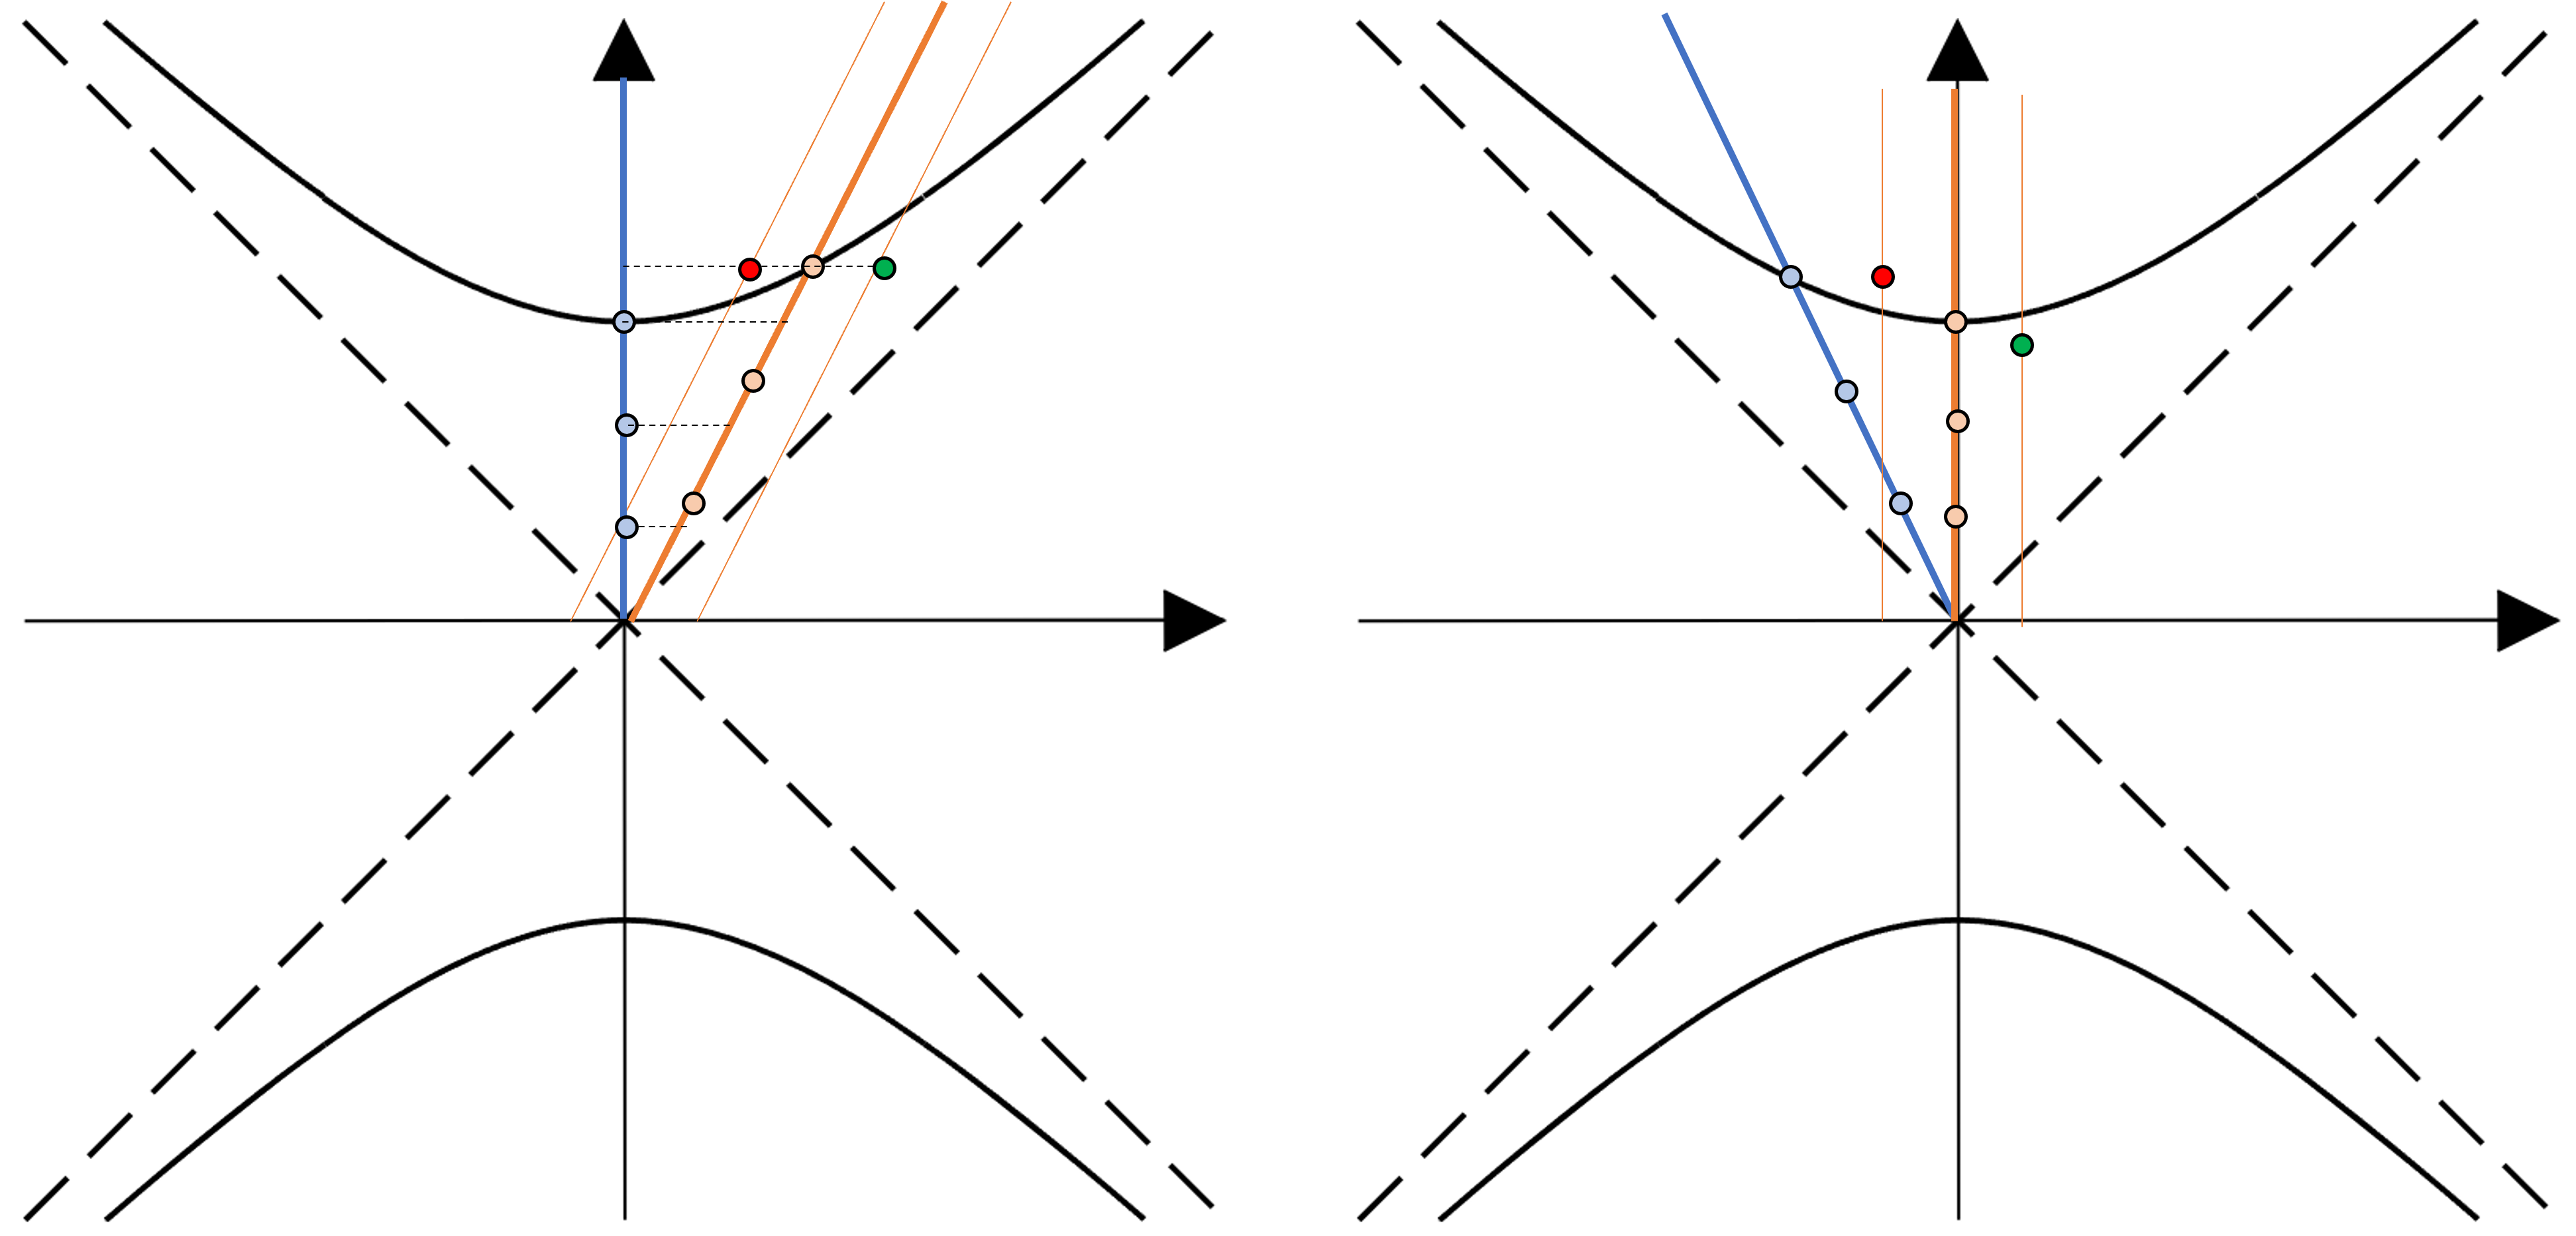
\includegraphics[scale=0.4]{figures/length-contraction-and-time-dilation.png}
	\caption{尺缩钟慢}
\end{figure}
如图,纵轴是 $ct$,横轴是 $x$,蓝色实线是 $K$ 系原点的时间线,橙色实线是 $K'$ 系原点的时间线。图中只画出来一条双曲线,但实际进行洛伦兹变换时,事件点是顺着紧密相接的一簇簇双曲线变化的。

\par 先考虑钟慢效应。图中蓝色圆圈在蓝色实线上均匀分布,表示 $K$ 系中的固有时在均匀流逝,橙色表示 $K'$ 系。我分别绘制了3个钟,代表各自的固有时,它们之间能够通过洛伦兹变换对应起来,要看出这种对应,我们可以考虑从左图到右图的连续变换过程。所以,很显然,在 $K$ 系到达1个单位时间时,$K'$ 系的钟还不到1个单位时间。这就直接说明了运动的物体时间变慢。

\par 再考虑尺缩效应。在 $K$ 系中为了测量载具长度,我同时测量车头(绿色圆圈)和车尾(红色圆圈)的坐标,作差,得到长度。但是在 $K'$ 系中,也就是右图,开车的司机就觉得很奇怪了,他诧异于为什么测量者先测量车头到观察者的距离,等车子走一段路了再测量车尾到他的距离,这么着去相减,肯定比司机觉得的真实车长要短呀!这就是运动的物体长度变短。上述讨论其实已经蕴含了同时的相对性。


\subsection{火车进隧道}

一列固有长度为 $l_{0}$ 的火车,进入固有长度恰好为 $l_{0}$ 的隧道。在隧道管理员的视角下,火车的长度减小,所以他能够看到火车完全进入隧道内部的状态,并在此时瞬时地关闭前后两个隧道门而不不会阻碍火车的运动。在火车驾驶员看来,隧道会变短,所以他能看到火车的车头和车尾同时在隧道前门后门之外,因而他能瞬时地在车头和车尾同时向天空发射烟花。

\par 聪明的你一定已经想到了,解决这个悖论的关键在于“同时的相对性”。比较精细缜密的图示,我放在了下面,其中包含了所有解决过程。注意下图只画了双曲线的两支,还有左右两支也应当绘制出来。另外,注意相邻两支双曲线的双曲旋转的方向。
\begin{figure}[H]
	\centering
	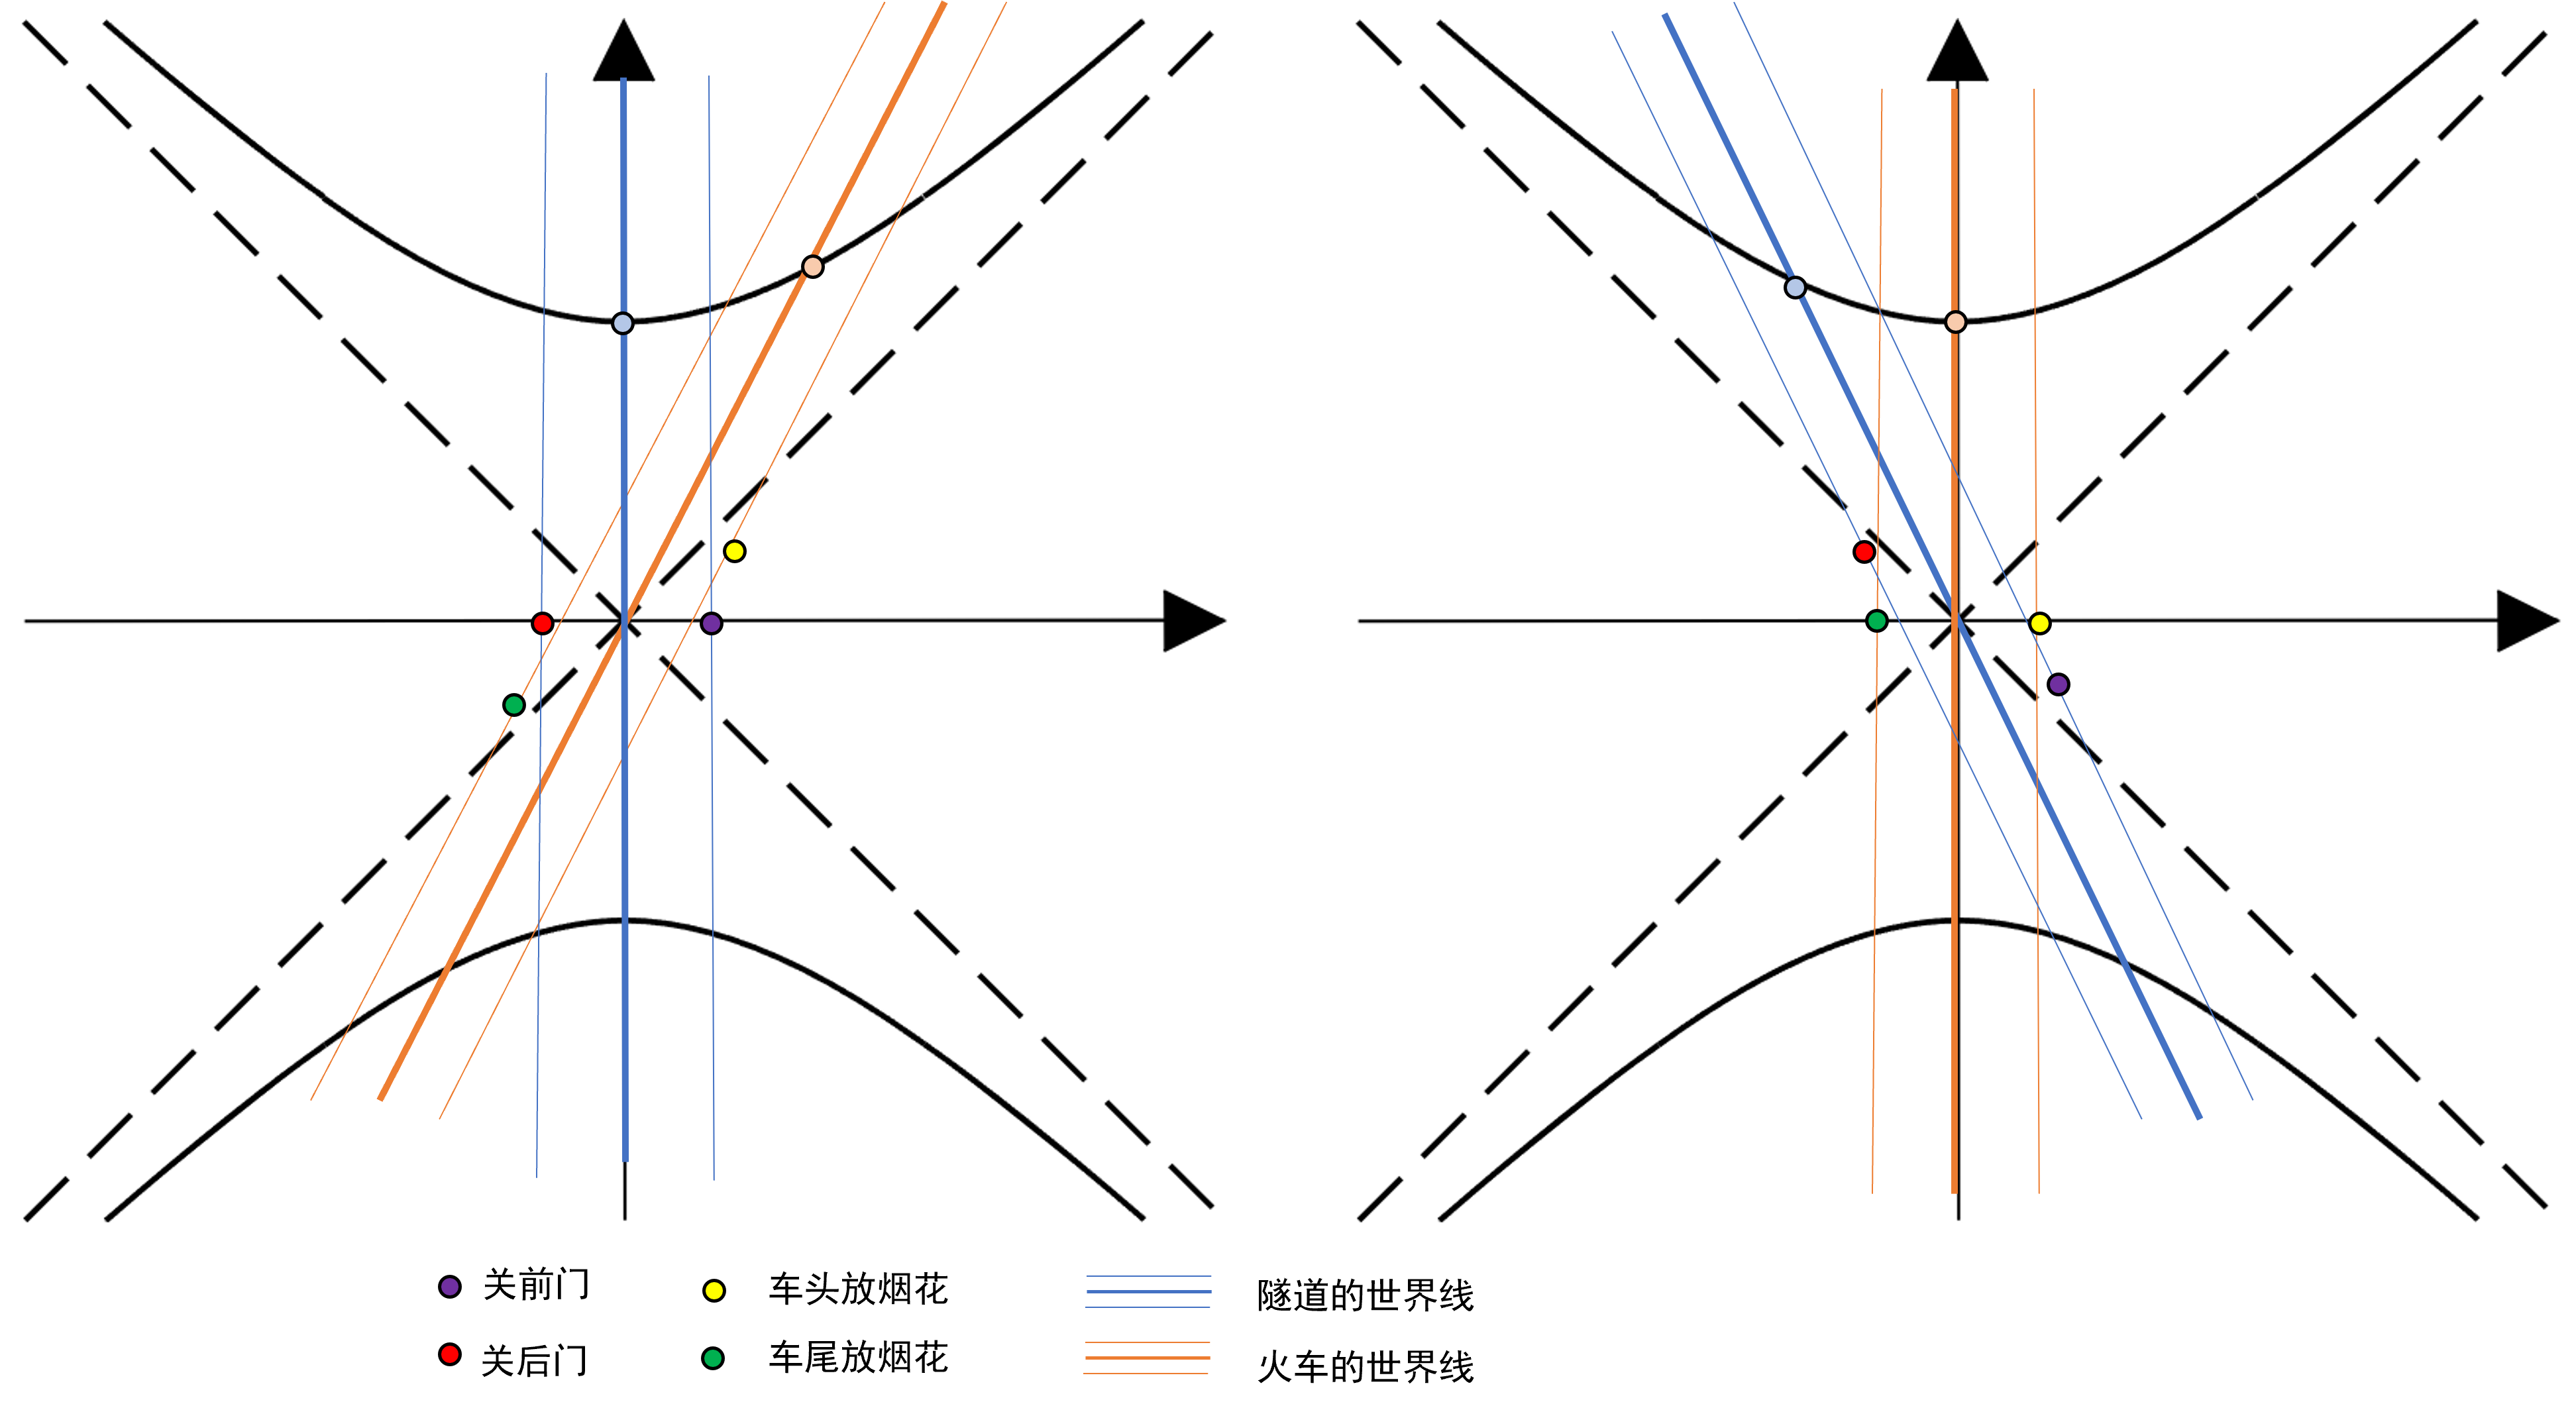
\includegraphics[scale=0.4]{figures/train-pass-tunnel.png}
	\caption{火车进隧道}
\end{figure}


\chapter{视觉效应}

我们所处的时空虽然是狭义相对论的时空,但是日常生活都是低速情形,我们几乎没有任何高速情形的视觉感知。我个人对此还是很好奇的,所以这部分来讨论一下:在近光速情形下,我们看到的世界会是什么样子的?

\par   或许第一反应是注意到洛伦兹收缩(尺缩效应),推测高速运动状态下,看到的景物都是被压缩的;在静止的时候,看到的高速运动的物体,也是被压缩的。

\par   其实,很多人都是这么想的,包括爱因斯坦本人也曾这样认为。俄国物理学家 George Gamov 在他的科普书籍 The New World of Mr Tompkins 中还据此做了栩栩如生的插图。

\begin{figure}[H]
	\centering
	\includegraphics[scale=0.5]{figures/contracted-world.png}
	\caption{压缩的世界}
\end{figure}

\par   但理论与实验都表明,这个考虑并不周全。洛伦兹收缩没有错,但它是个测量效应。视觉效应并不等于测量结果,视觉的形成首先需要满足:画面中的所有光线都是同一时刻到达眼睛的。这就意味着,虽然我们看到的画面中每一点发出的光线都是同时到达眼睛的,但是远处的物体反射或发出的光线要更早一点。

\section{转动}

先从最基本的几何体开始讨论。在讨论的时候,咱们抓住这一条原则:“远处的物体先发出光线,近处的物体后发出光线。”从最简单的情形开始讨论,即只考虑“远近”,暂不考虑角度。这相当于是我们将物体放在远处,此时物体到达人眼的光线可以近似认为是平行的。

\par   如图,一个边长为 $l$ 的正方体在远处做匀速运动,观察者是静止的,位于 $(x_{0},y_{0},0)$ 处。我们讨论在正方体刚好运动到 $(x_{0},y,0)$ 处(这种表达暗暗地将正方体视为质点)的情况下,我们看到的画面。

\begin{figure}[H]
	\centering
	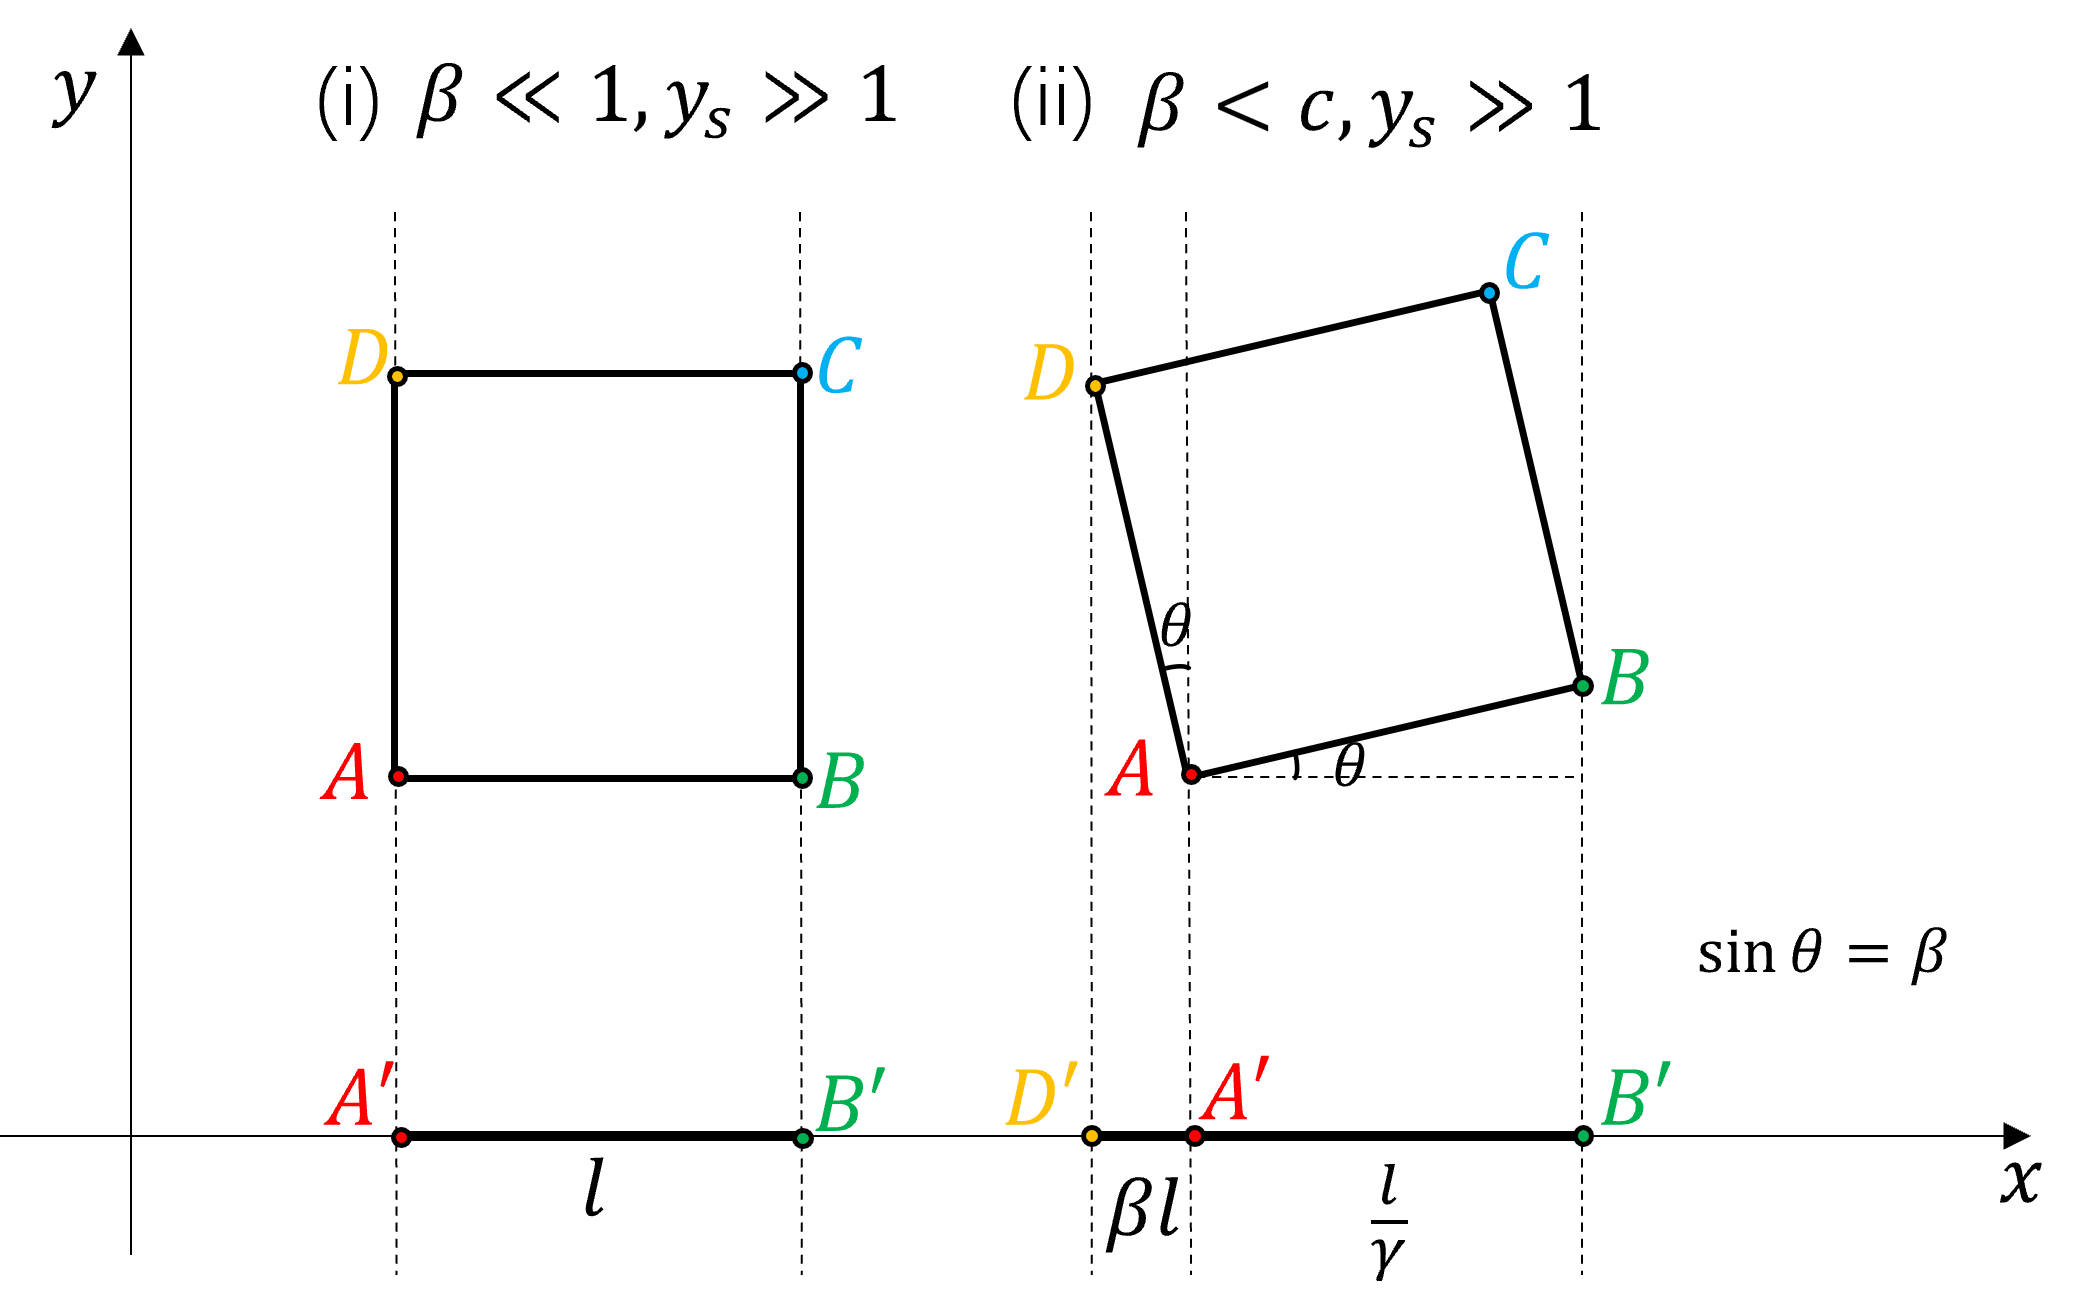
\includegraphics[scale=0.8]{figures/Terrell-rotation-square.png}
	\caption{运动的物体向外旋转}
\end{figure}

\par   在低速情形 (i) 下,显然我们只能看到正方形的 AB 边,长度几乎不变。而在高速情形 (ii) 下,AB 边发出的光比 CD 边早到达 $\Delta t=\frac{l}{c}$,那么当观察者接收到 AB 边发出的光线时,如果 CD 边发出的光线也能到达观察者,那么这束光反映的是 $\Delta t$ 之前的情况,也就是说通过这束光,我们以为 CD 边还没到达 AB 边所在的位置。而 AB 边会发生洛伦兹收缩,于是我们就会看到三个点:A, B, D.

\par   进一步定量讨论,我们发现,$D'A'=\beta l$,而 $A'B'=\sqrt{1-\beta^{2}}l$,如果引入几何参数 $\theta=\arcsin\beta$,那么

\begin{equation}
	\left\{\begin{aligned}
		A'B'&=AB\cos\theta \\
		D'A'&=DA\sin\theta
	\end{aligned}\right.
\end{equation}

这不正好相当于高速运动的正方形向外旋转了 $\theta=\arcsin\beta$ 的角度嘛!所以我们的眼睛就会认为,这个快速移动的正方形发生了旋转!看,我们在洛伦兹收缩的基础上,仅仅多考虑了光线的延迟,就得到了这样的物理图像!


\section{弯曲}

现在我们进一步精细化,去掉之前的一个假设:物体离观察者很远。如果物体离观察者有限远,那么光线就不能认为是平行光了,此时对光线延迟的计算就复杂了一些,不过仍然在初等几何的范畴内。

\par   如图,现在考虑立方体竖直方向的一条边,比如 $A^{t}A^{b}$ (t for top, b for bottom),在 $t_{1}$ 时刻,$A^{t}$ 的坐标为 $(x_{1},0,z)$,$A^{b}$ 的坐标为 $(x_{1},0,0)$;在 $t_{2}$ 时刻,$A^{t}$ 的坐标为 $(x_{2},0,z)$,$A^{b}$ 的坐标为 $(x_{2},0,0)$;观察者 $W$ (W for watcher) 位于 $(x_{2},y,0)$.

\begin{figure}[H]
	\centering
	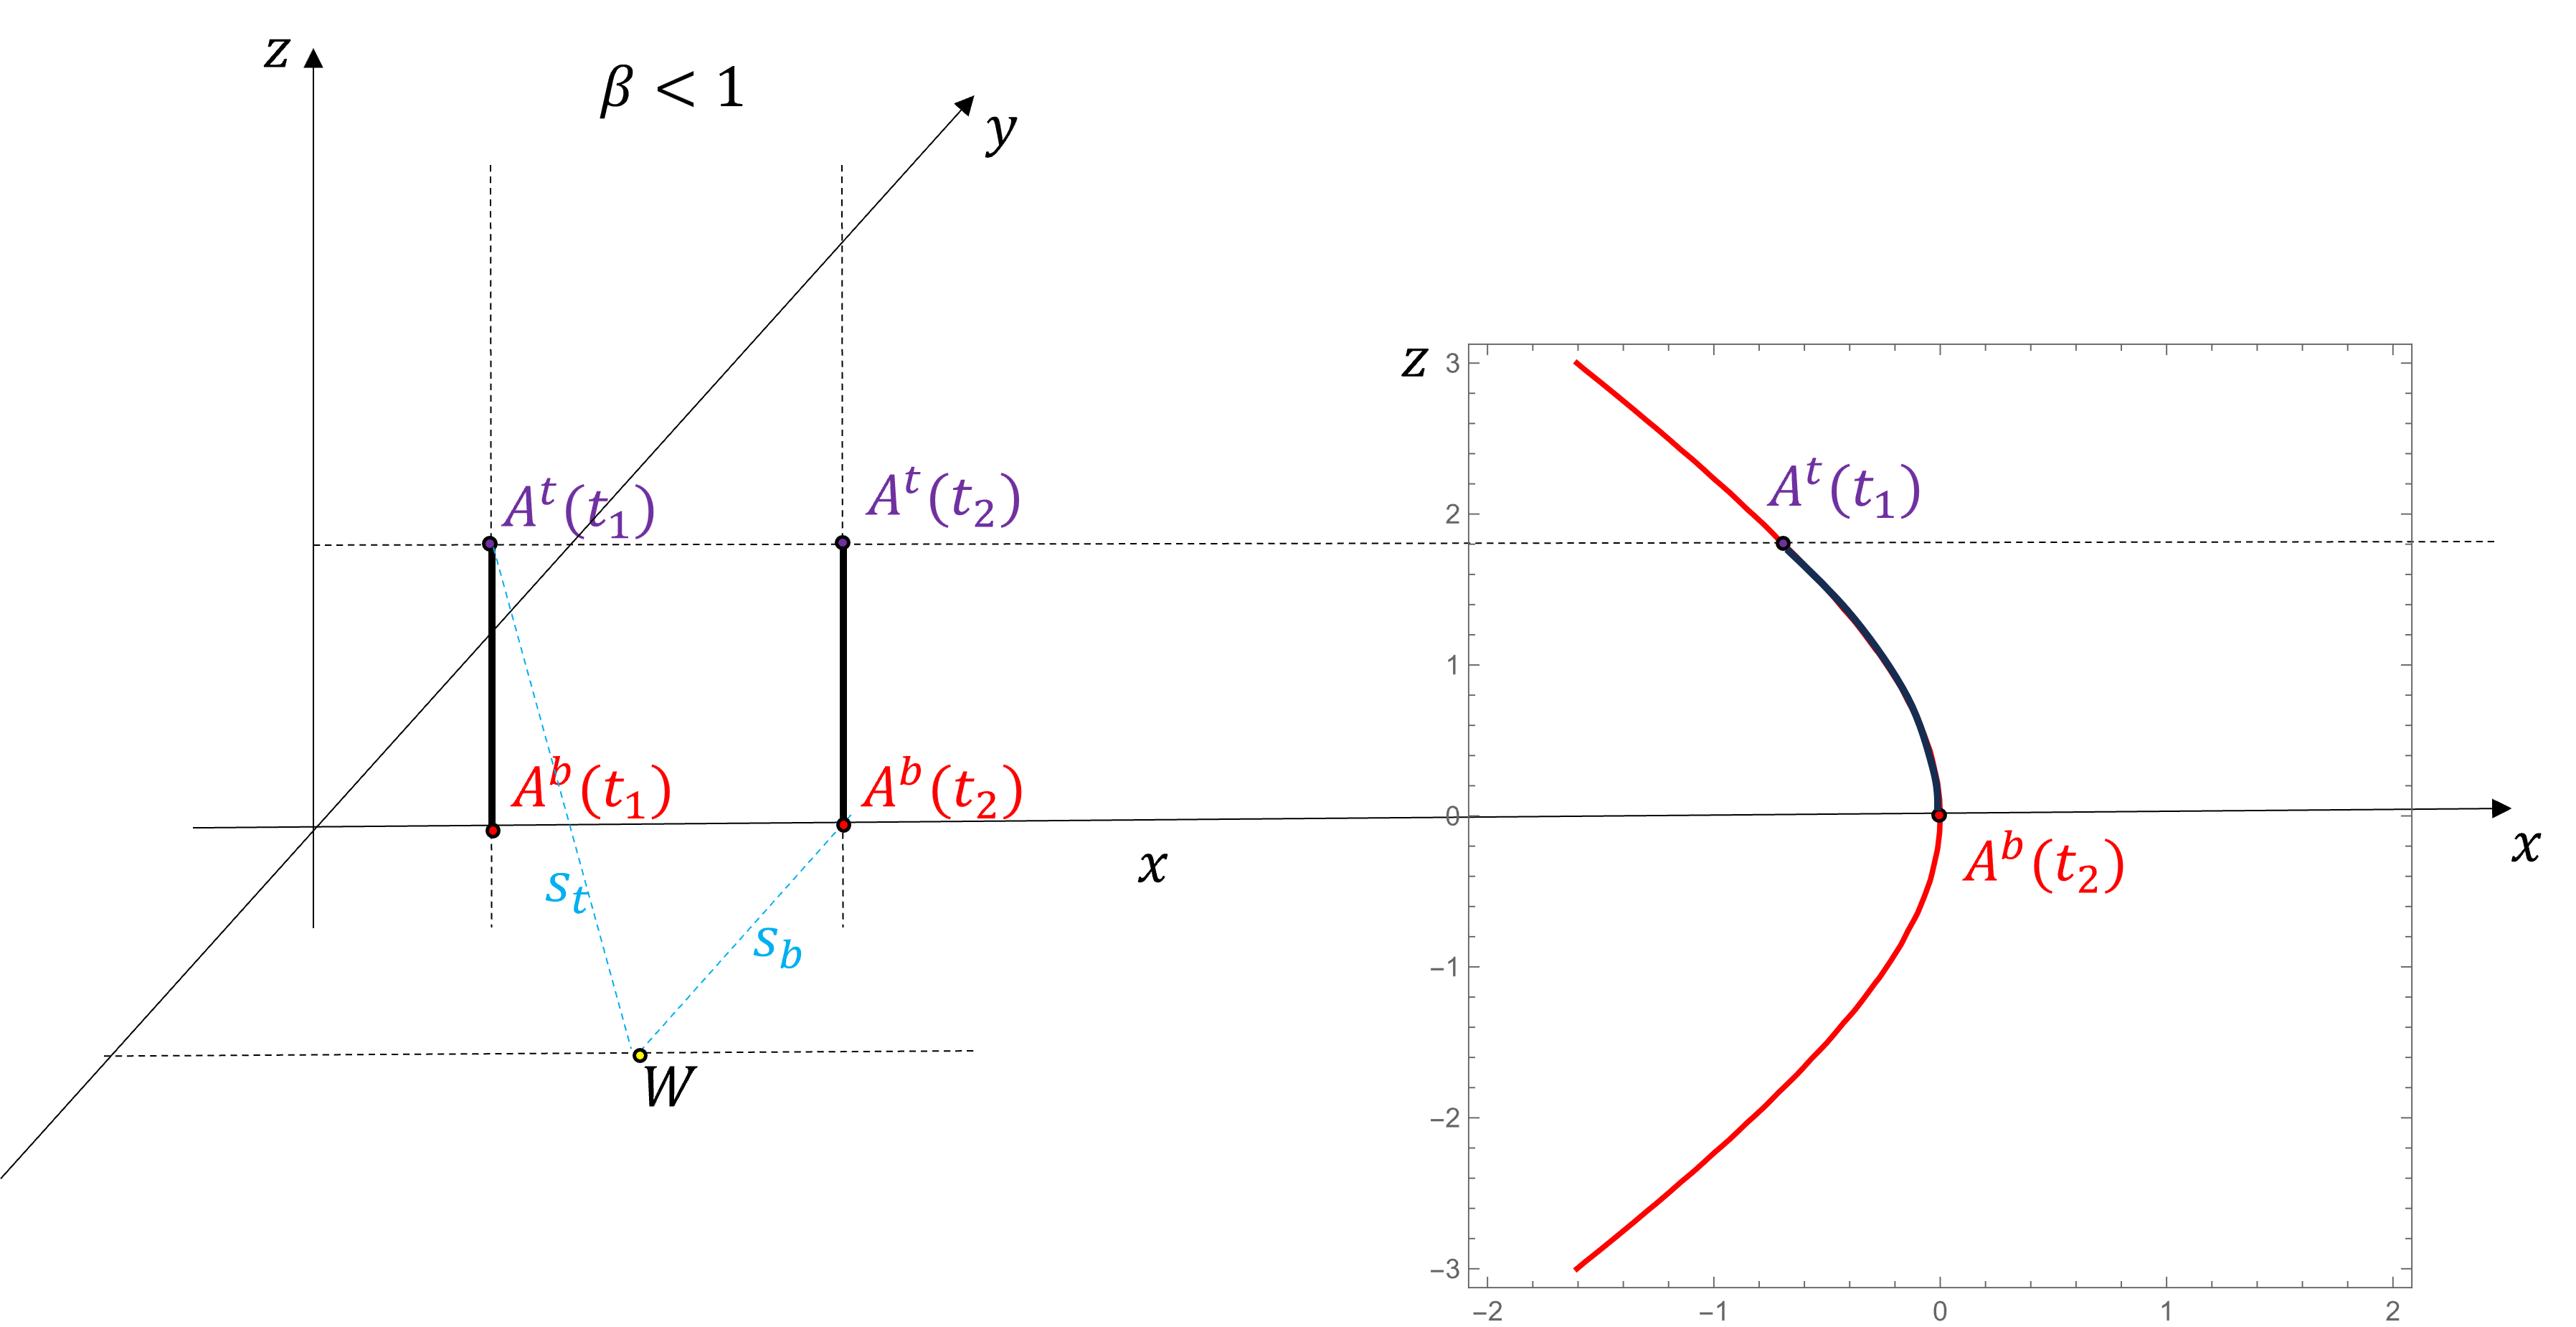
\includegraphics[scale=0.47]{figures/bending-distortion.png}
	\caption{弯曲畸变}
\end{figure}

\par   假设在时刻 $t$, $A^{b}$(在 $t_{2}$ 时刻)发出的光到达了 $W$,光走的路程记为 $s_{b}$. 那么对于成像原则,我们接收到的 $A^{t}$ 的光是更早之前($t_{1}$ 时刻)发出来的,光走的路程记为 $s_{t}$. 显然,有如下关系:

\begin{equation}
	\left\{\begin{aligned}
		s_{b}&=\qty|A^{b}(t_{2})W|=\qty|y| \\
		s_{t}&=\qty|A^{t}(t_{1})W|=\sqrt{(x_{2}-x_{1})^{2}+y^{2}+z^{2}} \\
		\Delta t&=\frac{x_{2}-x_{1}}{v}=\frac{s_{t}-s_{b}}{c}
	\end{aligned}\right.
\end{equation}

上面的方程组是好解的,但显然有一些参数和坐标是依赖于观察者的位置的。我们不妨将竖直棱上距离观察者最近的点(在此例为 $A^{b}$)在距离观察者最近时(在此例为 $t_{2}$)到观察者的距离记为 $d$(在此例为 $|y|$),将此时观察者或者说竖直棱的 $x_{2}$ 坐标规定为 $0$,将待求的 $x_{1}$ 记为 $x$,那么 $f(x,z)=0$ 可以写为

\begin{equation}
	z^{2}=\qty(\beta^{-2}-1)x^{2}-2d\beta^{-1}x
\end{equation}

这显然是一条二次曲线,或者说圆锥曲线。对于一般形式的二次曲线

\begin{equation}
	Ax^{2}+Bxy+Cy^{2}+Dx+Ey+F=0
\end{equation}

我们通过判别式 $\Delta=B^{2}-4AC$ 去判定曲线的形状,$\Delta>0$ 对应双曲线,$\Delta<0$ 对应椭圆,$\Delta=0$ 对应抛物线。在这里,显然有

\begin{equation}
	\Delta=\frac{1-\beta^{2}}{\beta^{2}}>0
\end{equation}

所以原本的竖直棱会变成双曲线。


\section{视长度}

在物体离观察者有限远的情况下,其实水平方向(沿速度方向)的线段的视距也会发生变化。这个除了跟洛伦兹收缩有关系,还跟光线延迟有关。

\begin{figure}[H]
	\centering
	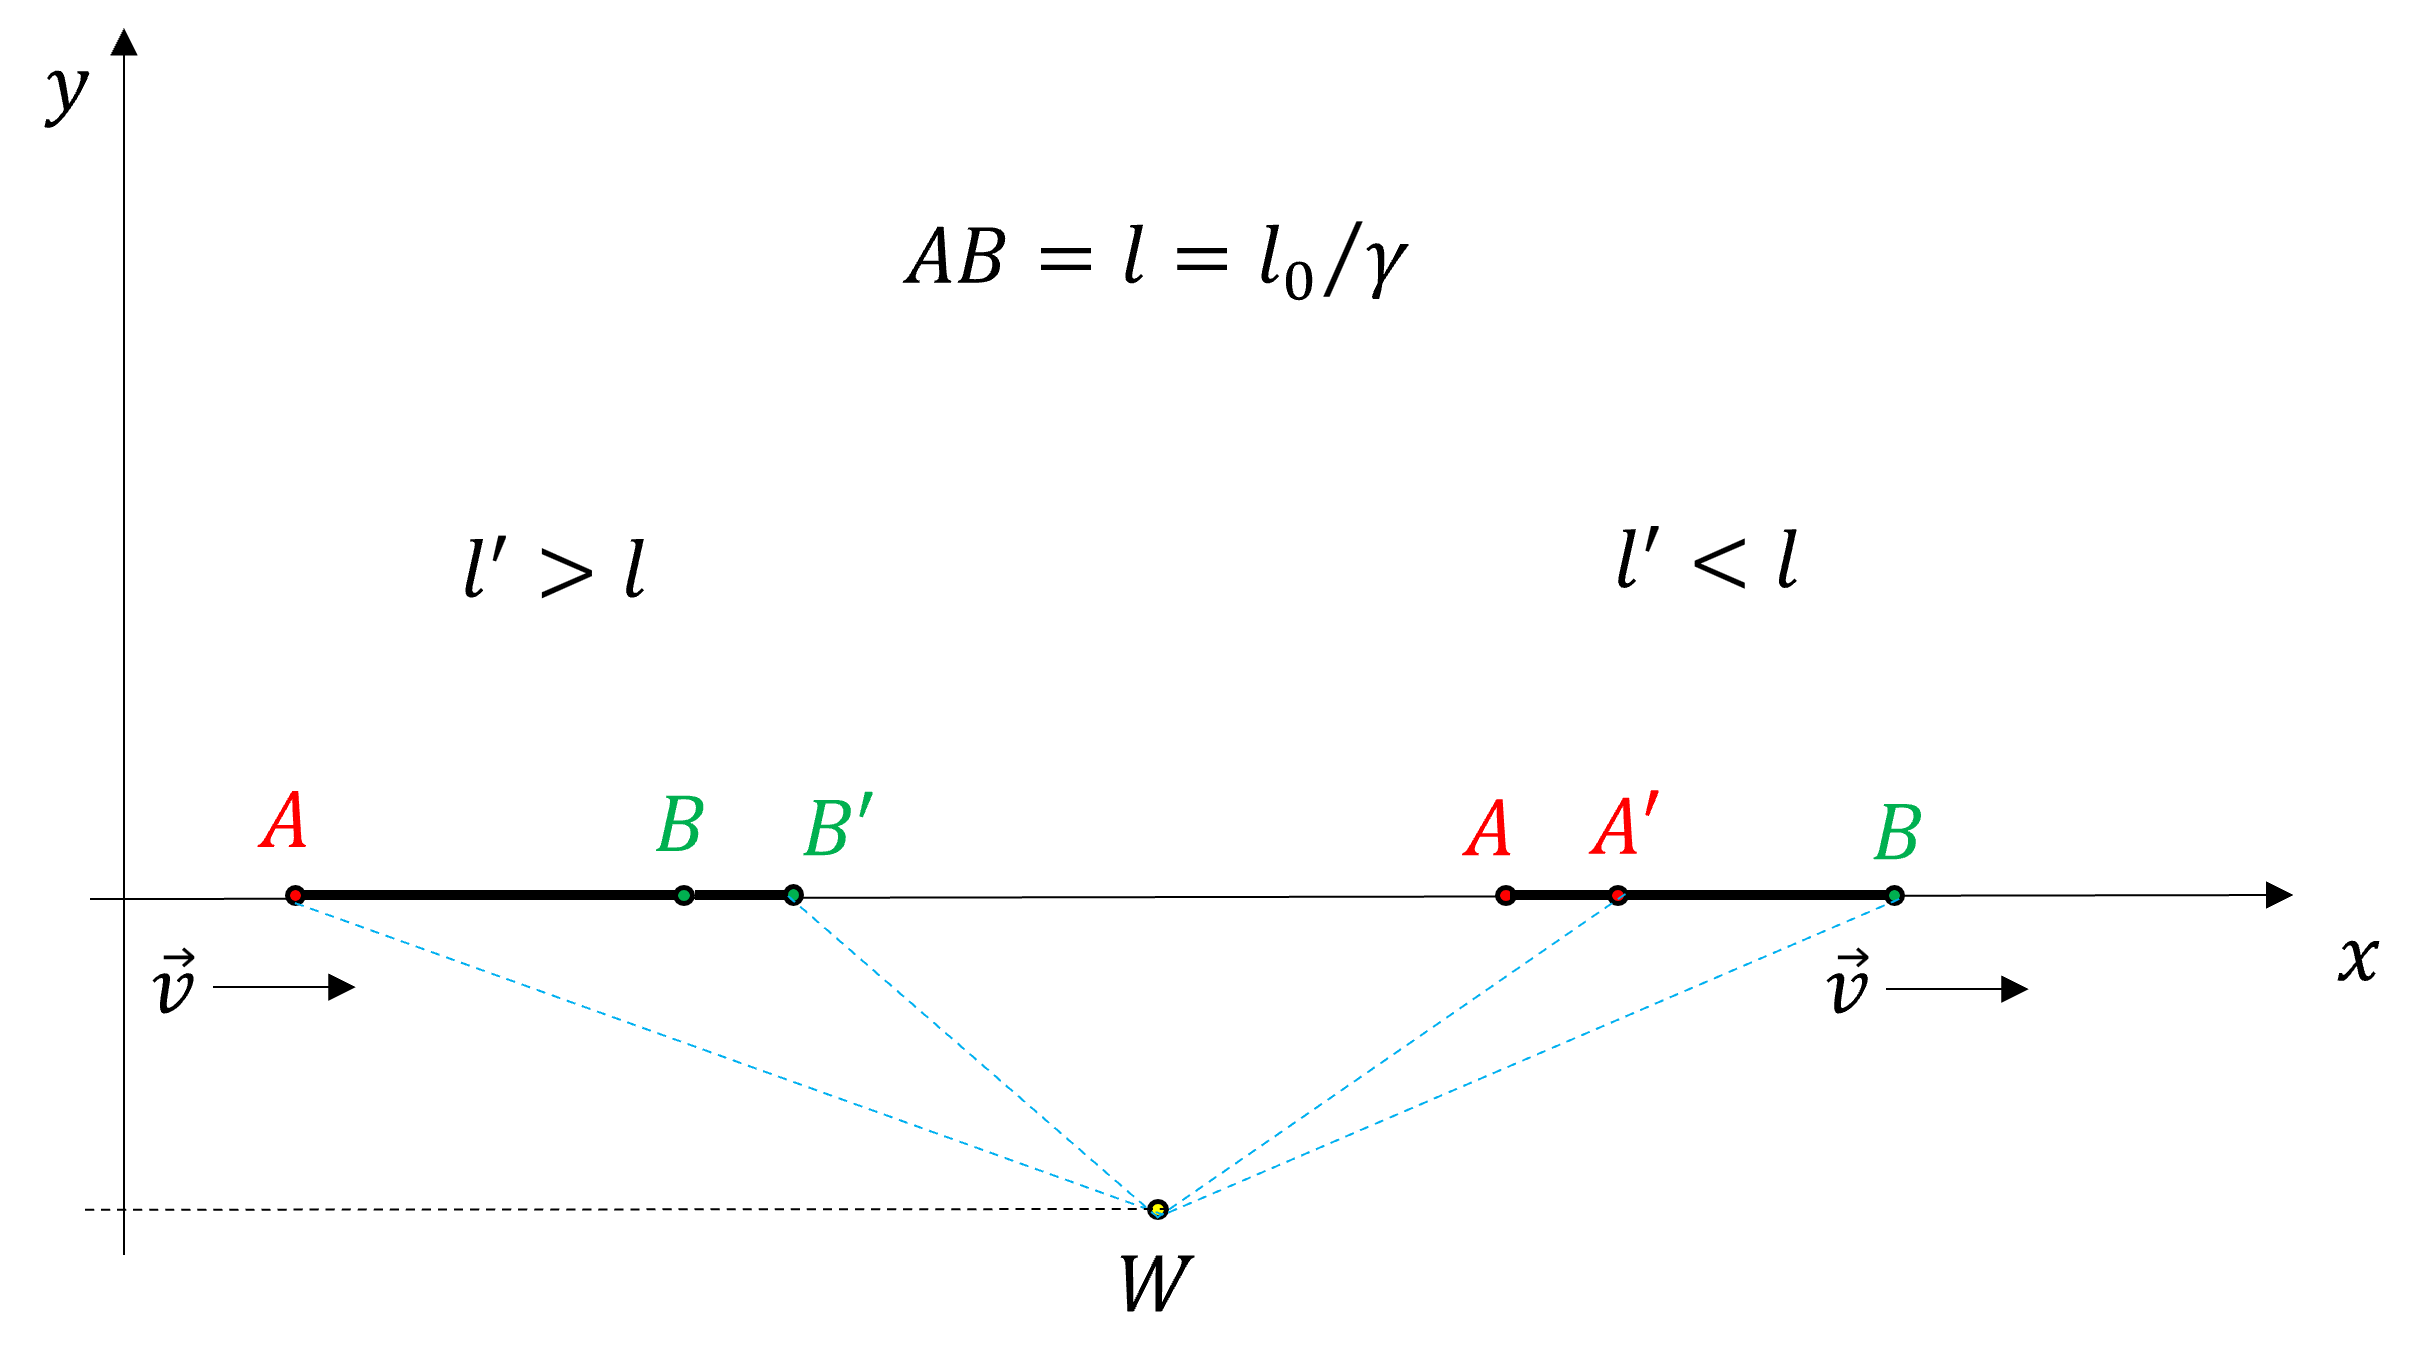
\includegraphics[scale=0.5]{figures/observing-length.png}
	\caption{视长度变化}
\end{figure}

所以,靠近观察者的图形会变长,远离观察者则会变短。这个结论很容易理解,计算也十分简单,这里不再赘述。

\par   到这里,读者可能会有两个问题:第一,光线延迟和洛伦兹收缩是独立的吗?第二,在相对论的时空中,不是说“同时具有相对性”嘛?那我前面那么多计算时间差的步骤,不需要再慎重一点?万一这种处理是没有考虑“同时具有相对性”这个性质呢?

\par   关于第一个问题,我的回答是肯定的。光线延迟完全是一个运动学的问题,是观察效应;而洛伦兹收缩是洛伦兹变换的推论,是测量效应,两者有着本质的区别,当然是独立的,因而也是需要分别考虑的。

\par   关于第二个问题,这个其实更为要紧,也能一定程度上补充我对第一个问题的回答。什么叫“同时的相对性”?在 $K$ 系中同时发生的事情,在 $K'$ 系中却并不同时;在 $K$ 系中相隔 $\Delta t$ 的两个事件,在 $K'$ 系中却并不是。那么,同时的相对性是以什么为基础的?它有一个默认的基础,就是,在任意参考系中,“同时”这个概念还是成立的,垂直于 $t$ 轴的直线还是存在的,并且很多,根本不受洛伦兹变换的影响、根本不受双曲几何的影响。所以,在不涉及参考系变换时,大胆地使用“同时”这个概念吧!这里光线延迟的计算跟小学时学到的计算方法是一致的。

\par   嘿嘿,你以为我不慎重,其实俺这叫艺高人胆大!

综上所述,在高速运动的情景下,我们会看到如下情形。注意结合上面提到的几个效应,仔细鉴赏。

\begin{figure}[H]
	\centering
	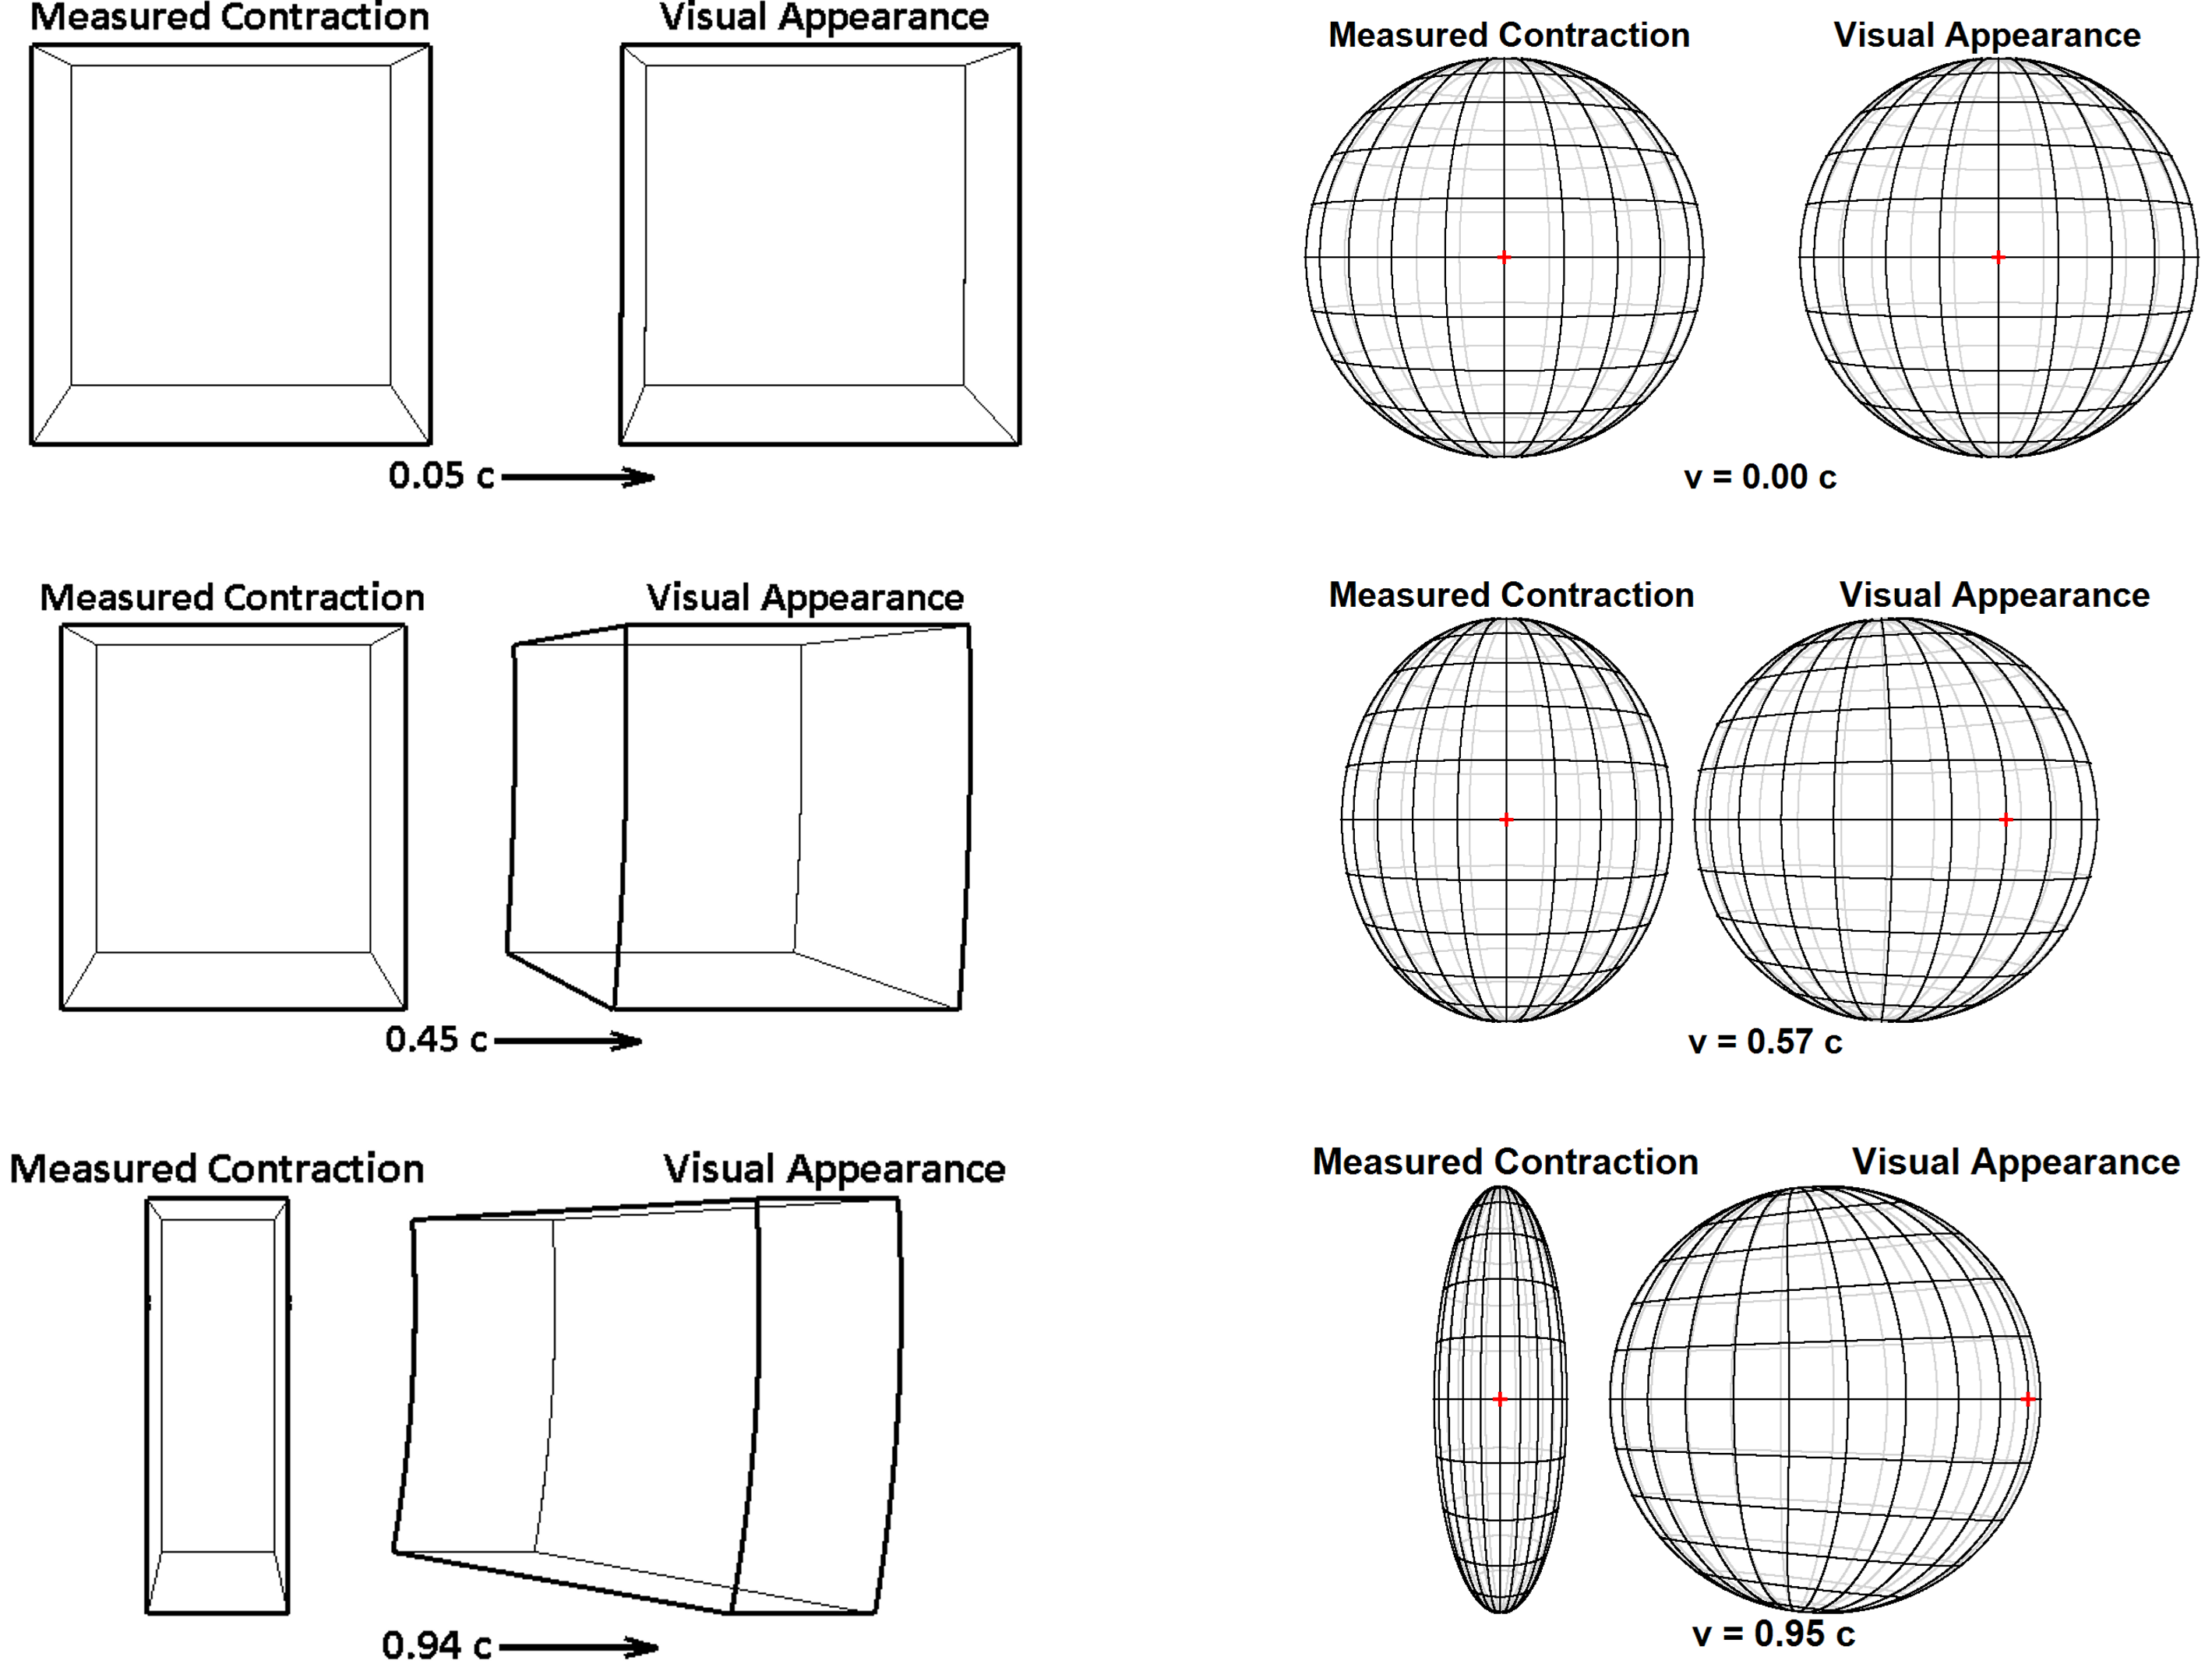
\includegraphics[scale=0.6]{figures/Terrell-rotation.png}
	\caption{Terrell旋转}
\end{figure}

\section{多普勒效应}

我们的世界,怎么能全是几何而没有色彩?说到色彩,那就不得不提到多普勒效应了!在伽利略变换下的时空里面,我们也推导过多普勒效应,具体如下

\begin{equation}
	f'=\frac{u+v}{u-v}f
\end{equation}

其中 $u$ 是波速,$v$ 是观察者和波源之间的相对速度,如果观察者有速度,就体现在分子上;如果波源有速度,就体现在分母上;两者同时移动,那么分子分母都乘上来。当然,只有纵向的相对速度才有这种频移。

\par   在狭义相对论的时空中,情况有所不同了。还记得咱们之前说过波的相位 $\phi=\omega t-\vb*{k}\cdot\vb*{x}$ 是一个洛伦兹标量吧,它可以表示成 $\phi=k^{\mu}x_{\mu}$的形式,其中 
\begin{equation}
	k^{\mu}=\qty(\frac{\omega}{c},\vb*{k})
\end{equation}
显然是一个逆变4-矢量,因为它和 $x_{\mu}$ 的缩并是洛伦兹标量嘛。既然是洛伦兹张量,那么电磁波的4-波矢就满足洛伦兹变换 $k'^{\mu}=\Lambda^{\mu}_{\nu}k^{\nu}$,或者我们采用式\eqref{e1.11}的形式,写为
\begin{equation}\label{Doppler}
	\frac{\omega'}{c}=\gamma\qty(\frac{\omega}{c}-\vb*{\beta}\cdot\vb*{k})\quad\Leftrightarrow\quad\omega'=\gamma\omega(1-\beta\cos\theta)
\end{equation}
上式利用了光在真空中的色散关系 $|\vb*{k}|=\frac{\omega}{c}$. 根据式\eqref{Doppler}可以得到纵向多普勒效应和横向多普勒效应
\begin{equation}
	\left\{\begin{aligned}
		\omega'&=\omega\sqrt{\frac{1-\beta}{1+\beta}}\\
		\omega'&=\frac{\omega}{\sqrt{1-\beta^{2}}}
	\end{aligned}\right.
\end{equation}
其中纵向多普勒发生了变化,而横向多普勒效应更是完完全全的狭义相对论的产物。比如我们向左移动,会发现左边的视野“变蓝”,右边的视野“变红”。

\par   由于光具有波动性,所以会发生多普勒效应,靠近物体时发生蓝移,远离时红移。另外,由于光具有粒子性,靠近观察者的物体会变得更亮,远离时变暗。

\par   强烈推荐大家玩一玩 MIT 制作的游戏《A Slower Speed of Light》,里面集合了上面提到的所有视觉效应!

\begin{figure}[H]
	\centering
	\includegraphics[scale=0.4]{figures/a-slower-speed-of-light.png}
	\caption{https://gamelab.mit.edu/games/a-slower-speed-of-light/}
\end{figure}

\end{document}